 \documentclass[12pt]{book}

% Set up data if you need to add a package, go here
%Adapted from Adapted from UWA Engineering Final Year Project.
\usepackage{cite} 
\usepackage{floatrow}
\usepackage[utf8]{inputenc}
\usepackage[x11names,dvipsnames,svgnames,table]{xcolor}
\usepackage{comment}
\usepackage{afterpage}
\usepackage[left=3.5cm,right=2cm,top=3.5cm,bottom=2cm]{geometry}
% general incantations
\usepackage{gensymb}
\usepackage{afterpage}
\usepackage{physics}
\usepackage{graphicx}
\usepackage{placeins}
\usepackage{pdfpages}
\usepackage{array}
\usepackage{booktabs}
\usepackage{subcaption}
\usepackage{rotating}
\usepackage{tikz}
\usepackage{float}

\usepackage{parskip}
\usepackage{lscape}

\usepackage{verbatim}

%Automated appendices

%language settings
\usepackage[utf8]{inputenc}
\usepackage[australian]{babel}
\usepackage{titlesec}
 \usepackage{hyperref}
%maths stuff
\usepackage{amsmath}
\usepackage{mathtools}
\usepackage{amsfonts}
\usepackage{amssymb}
\usepackage{mathrsfs}
\usepackage{nccmath}
%lists
\usepackage{enumitem}

%working collaboratively
\usepackage[backgroundcolor=yellow]{todonotes}



%glossary for acronyms
\usepackage[acronym,nonumberlist,toc,section=subsection,numberedsection=nolabel]{glossaries} 
\makeglossaries

%line spacing
\linespread{1.25}


\newcommand\blankpage{
    \null
    \thispagestyle{empty}
    \addtocounter{page}{0}
    \newpage
    }
    
\titleclass{\part}{top}
\titleformat{\part}[display]
  {\normalfont\huge\bfseries}{\centering\partname\ \thepart}{20pt}{\Huge\centering}
\titlespacing*{\part}{0pt}{50pt}{40pt}
\titleclass{\chapter}{straight}
\titleformat{\chapter}[display]
  {\normalfont\huge\bfseries}{\chaptertitlename\ \thechapter}{20pt}{\Huge}
\titlespacing*{\chapter} {0pt}{50pt}{40pt}

\begin{document}
\newcommand\numberthis{\addtocounter{equation}{1}\tag{\theequation}}

\raggedbottom


\thispagestyle{empty}
\setlength\headheight{0pt} 
\begin{center}

\begin{center}

\includegraphics[width=1\linewidth]{images/logo.jpg}            
\end{center}    

  \vspace{3 cm}

        {\Large\bfseries  ``Interaction-free measurements of different absorbers''\par}

        \vspace{0.5cm}
        {\Large\itshape by \\ \bfseries Gerardo José Suárez Rodríguez \par \par}
        

\vspace{2cm}


Master of Science, \\ Physics\\
Supervised by\par
Dr. Alonso Contreras Astorga  \\
Dra. Sara Guadalupe Cruz y Cruz\\


\vspace{1cm}
\large
\today

\end{center}

\clearpage

\tableofcontents
\addtocontents{toc}{\protect\thispagestyle{empty}}
\pagebreak
\pagenumbering{Roman}

\begin{comment}
\chapter*{Declaration}
I hereby certify that the material, which I now submit for assessment on the programs of study leading to the award of Master of Science, is entirely my work and has not been taken from the work of others except to the extent that such work has been cited and acknowledged within the text of my work. No portion of the work contained in this thesis has been submitted in support of an application for another degree or qualification to this or any other institution.
\addcontentsline{toc}{section}{Declaration}

\vspace{2cm}
\begin{flushright}
-----------------------------------\\
Gerardo Suárez\\
\today
\end{flushright}
\pagebreak

%List of figures and tables, automatic from thesis.
\addcontentsline{toc}{section}{List of Figures}
\listoffigures\newpage


\addcontentsline{toc}{section}{List of Tables}
\listoftables\newpage

\end{comment}

\chapter*{Acknowledgements}
\thispagestyle{plain}
Most figures were made using svgs from flaticom.com, the component library of Alexander Franzen and the noun project
\addcontentsline{toc}{section}{Acknowledgements}

\pagebreak



\blankpage{}
\chapter*{Resumen}
\thispagestyle{plain}
\addcontentsline{toc}{section}{Resumen}

\pagebreak



\blankpage{}
\chapter*{Abstract}
\thispagestyle{plain}
This is done at the end of the project
\addcontentsline{toc}{section}{Abstract}


\pagebreak


\blankpage{}

\chapter*{Introduction}
\thispagestyle{plain}
\addcontentsline{toc}{section}{Introduction}
\pagebreak
\blankpage{}

\pagenumbering{arabic}

\chapter[SPDC]{Spontaneous parametric \\ down conversion}



In this section, we will explore the quantum theory of Spontaneous Parametric Down-Conversion (SPDC), following the approach taken in \cite{procopio,multiphoton}. The SPDC phenomenon is a process in which an intense laser beam called pump beam, is incident to a nonlinear crystal. Occasionally, one photon of the pump beam is annihilated in the crystal and two photons which are known as signal and idler photons, of lower frequencies, are created preserving the total energy and linear momentum.

Considering that the energy is given by $E=\hbar w$, where $w$ is the angular frequency, and the linear momentum is ($\mathbf{p}=\hbar \mathbf{k}$), where $\mathbf{k}$ is the wave vector, the conservation law reads as:

\begin{equation}
w_{p}=w_{s}+w_{i}, \qquad \mathbf{k}_{p}=\mathbf{k}_{s}+\mathbf{k}_{i}, \label{conservation}
\end{equation}

where the sub-indices p, i,s refer to pump, signal and idler respectively. This is the name often used in the literature for each of the photons in the process. Pump refers to the photons of the laser beam. The signal term concerns the photon that undergoes the physical process under consideration, while the idler one is attributed to the second photon that witnesses the presence of the first one.

There are three types of SPDC, namely, type-0, type-I, and type-II. Each type of SPDC is defined by the polarization of all the photons involved in the process. In type-0 SPDC, all converted photons have the same polarization which is the same as the pump's annihilated photon.

\begin{figure}[h!]
\centering
\begin{subfigure}[b]{0.45\linewidth}
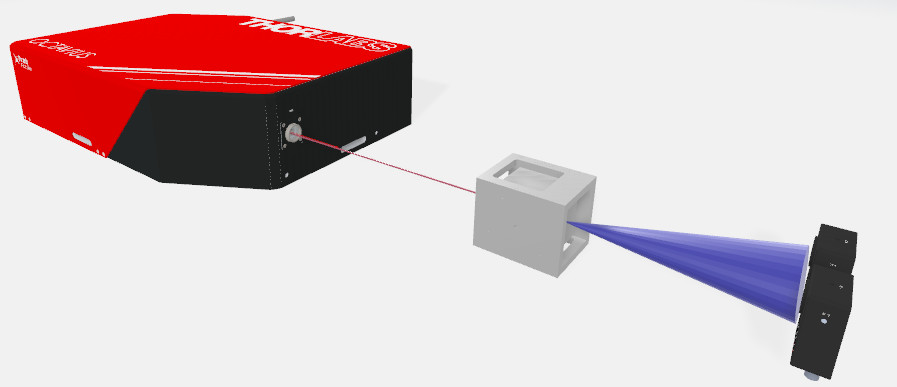
\includegraphics[width=\linewidth,height=2.8 cm]{images/TypeI.jpg}
\caption{SPDC type I}
\label{fig:type1}
\end{subfigure}
\begin{subfigure}[b]{0.45\linewidth}
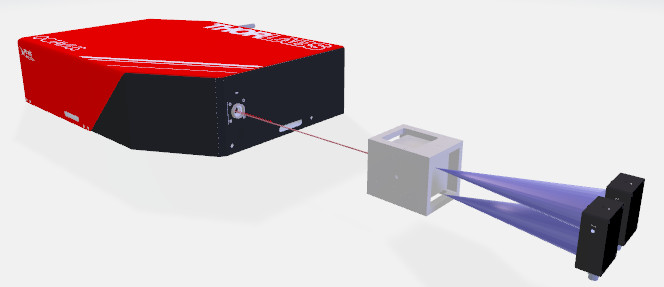
\includegraphics[width=\linewidth,height=2.8 cm]{images/typeII.jpg}
\caption{SPDC type II}
\label{fig:type2}
\end{subfigure}
\caption{An illustration of the SPDC type I and II processes, a laser incident on a non-linear crystal and photons coming out of it along cones.}
\label{fig:SPDC}
\end{figure}

Next, in type-I, both converted photons have the same polarization, and it is orthogonal to that of the pump beam. In SPDC type I, both photons travel along the same cone (photons come out of the crystal in a cone shape, this is a spontaneous process and a given photon can be anywhere on the surface of said cone).

Finally, in SPDC type-II the polarization of converted photons are orthogonal, one of them the signal is the same polarization as the pump's. In this type of SPDC, each photon travels along its own cone.

In this work, we are mainly concerned with the SPDC type-I process.

We will start our description of the SPDC process by considering the quantized electric field operator which can be written as:

\begin{align}
\textbf{E}(\textbf{r},t)&=\textbf{E}^{(+)} (\textbf{r},t) + \textbf{E}^{(-)} (\textbf{r},t), \label{fiel+}
\end{align}

with

\begin{align}
\textbf{E}^{(+)} (\textbf{r},t)&=\frac{i(2 \pi \hbar w)^{\frac{1}{2}}}{\sqrt{V}} \sum_{\textbf{k},\nu}  \mathbf{a}_{\textbf{k},\nu} \mathbf{e}_{\textbf{k},\nu} e^{i(\textbf{k.r}-wt)}=[\textbf{E}^{(-)} (\textbf{r},t)]^{\dagger}, \label{quanfield}
\end{align}

where $w$ is the frequency of the electric field, $\mathbf{k}$ is the wave vector of all modes with defined linear momenta, we sum over this modes and polarizations as part of the canonical quantization process where we make a spatial Fourier expansion \cite{grynberg}, $\mathbf{e}_{\textbf{k},\nu}$ where $\nu=1,2$, is the polarization vector for a normal mode of wave vector $\mathbf{k}$ and defined polarization labeled by $\nu$, $\mathbf{a}_{\textbf{k},\nu}$ is the photon annihilation operator of the mode with wave vector $\mathbf{k}$ and polarization given by $\nu$. Finally, $V$ is the quantization volume, when we quantize we consider a finite volume (usually a cube) such that $k_{m}=\frac{2 \pi n_{m}}{L}$ where $m=x,y,z$ and $L$ is the length of said cube, the annihilation and creation operators must obey:

\begin{equation}
[\mathbf{a}_{\textbf{k},\nu},\mathbf{a^{\dagger}}_{\textbf{k},\nu}]=\delta_{\nu \nu'}\delta_{\textbf{k}\textbf{k'}},
\end{equation}

where $\delta_{ab}$ is the Kronecker's delta. The creation and annihilation operators act on the Fock basis as:

\begin{equation}
    \mathbf{a}_{\textbf{k},\nu}\ket{n}=\sqrt{n}\ket{n-1},\qquad
    \mathbf{a}_{\textbf{k},\nu}\ket{n}=\sqrt{n+1}\ket{n+1}.\label{Fock}
\end{equation}

The field operator $\textbf{E}^{(+)} (\textbf{r},t)$ acting on $\ket{0}$ which means the absence of photons of wave vector $\mathbf{k}$ and polarization $\nu$ is given by:

\begin{equation}
\textbf{E}^{(+)} (\textbf{r},t)\ket{0}=0,
\end{equation}

 with the adjoint relation:

\begin{equation}
\bra{0}\textbf{E}^{(-)} (\textbf{r},t)=0.
\end{equation}

The Hamiltonian operator of a quantized electromagnetic field can be written as \cite{jackson}:

\begin{equation}
H=\frac{1}{2}\int_{V} d^{3}r (\mathbf{D \cdot E}+\mathbf{H \cdot B}),
\end{equation}

where $\textbf{D}$ and $\textbf{H}$ are the electric displacement and the magnetic field operators, respectively. These are given in terms of the electric field $\textbf{E}$ and the magnetic flux $\textbf{B}$ by means of the constitutive relations (with $\epsilon_{0} $ being the permittivity and $\mu_{0}$ the permeability of free space):


\begin{align}
\textbf{D}= \epsilon_{0} \textbf{E}+\textbf{P},\\
\textbf{H}=\frac{\textbf{B}}{\mu_{0}}-\textbf{M},
\end{align}

where $\mathbf{P}$ is the electric polarization (the polarization) and $\mathbf{M}$ is the magnetic polarization (the magnetization) of the optical medium of interest (a non-linear crystal). In this work, we will neglect $\textbf{M}$ because we will assume that the laser beam is not intense enough to magnetize the crystal. Hence, the Hamiltonian becomes:

\begin{equation}
H=\frac{1}{2}\int_{V} d^{3}r \left(\epsilon_{0}\mathbf{E \cdot E}+\mathbf{E \cdot P}+\frac{\mathbf{B \cdot B}}{\mu_{0}} \right).
\end{equation}


As described in \cite{boyd}, while in linear optics polarization is often described by $\mathbf{P}(t)=\epsilon_{0} \chi^{(1)}\mathbf{E}(t)$, in nonlinear optics this equation is generalized by expressing the polarization as a power series of the field strenght:

\begin{equation}
\mathbf{P}(t)=\epsilon_{0} \left( \chi^{(1)}\mathbf{E}(t)+\chi^{(2)}\mathbf{E}^{2}(t)+\chi^{(3)}\mathbf{E}^{3}(t)+.... \right)=\mathbf{P}^{(1)}(t)+\mathbf{P}^{(2)}(t)+\mathbf{P}^{(3)}(t)+...
\end{equation}

 We will consider the polarization to have nonlinear components and the linear term to be included in a term we will call $H_{0}$
 
\begin{equation}
 H_{0}=\frac{1}{2}\int_{V} d^{3}r \left(\epsilon_{0}\mathbf{E \cdot E}+\mathbf{E} \cdot \mathbf{P^{(1)}}+\frac{\mathbf{B \cdot B}}{\mu_{0}} \right),
\end{equation}

  the zeroth order term or polar term is negligible because we are not considering polar media, the main contributor to the process is the second-order term in the nonlinear expansion which we will include in $H_{I}$, we will consider higher orders to be negligeable:


\begin{equation}
H_{I}=\frac{1}{2} \int_{V} d^{3}r \textbf{E} \cdot \textbf{P}^{(2)}, \label{Hi}
\end{equation}

where

\begin{equation}
P_{i}^{(2)} (\mathbf{r},t)=\int_{0}^{\infty}dt_{1}\int_{0}^{\infty}dt_{2} \chi_{ijk}^{(2')}(t-t_{1},t-t_{2}) E_{j}(\textbf{r},t_{1}) E_{k}(\textbf{r},t_{2}), \label{polariza}
\end{equation}

and $\chi_{ijk}^{(2')}$ is related to the second-order nonlinear susceptibility and represents the response of the medium to the second power of the electric field. By substituting Eq. \ref{polariza} in  Eq. \ref{Hi} and separating the field operators into its the creation and annihilation components, the interaction Hamiltonian $H_{I}$ turns into (we dropped the dependence of the fields to have a compact expression):

\begin{align*}
&H_{I}=\frac{1}{2} \int_{V}\int_{0}^{\infty}dt_{1}\int_{0}^{\infty}dt_{2} \chi_{ijk}^{(2')}(t-t_{1},t-t_{2}) \left( E_{i}^{(+)}E_{j}^{(+)}E_{k}^{(+)}+E_{i}^{(-)}E_{j}^{(+)}E_{k}^{(+)}\right.\\
&+ E_{i}^{(-)}E_{j}^{(-)}E_{k}^{(+)}+E_{i}^{(+)}E_{j}^{(-)}E_{k}^{(+)}+E_{i}^{(+)}E_{j}^{(+)}E_{k}^{(-)}+E_{i}^{(-)}E_{j}^{(+)}E_{k}^{(-)}\\
&+ \left.E_{i}^{(-)}E_{j}^{(-)}E_{k}^{(-)}+E_{i}^{(+)}E_{j}^{(-)}E_{k}^{(-)}  \right). \label{muchoscampos} \numberthis
\end{align*}

Since the SPDC process involves the annihilation of one photon of the pump beam and the creation of two photons of lower frequency, the only terms of Eq. \ref{muchoscampos} which are compatible with such phenomenon are those including $E_{i}^{(+)}E_{j}^{(-)}E_{k}^{(-)}$ (according to Eq. \ref{fiel+} the label $(+)$ is associated with the annihilation of photons and $(-)$ to their creation) and its Hermitian conjugate describing the reverse process. The other terms represent processes that do not preserve energy  so they will not be considered. Thus, the Hamiltonian $H_{I}$ reduces to:

\begin{equation}
H_{I}=\int_{V} d^{3}r \chi_{ijk}^{(2)}(w_{j},w_{k}) (E_{i}^{(+)}E_{j}^{(-)}E_{k}^{(-)})+\mathrm{H.c}, \label{Hi2}
\end{equation}

where  $\mathrm{H.c}$ means Hermitian conjugate and we redefined:


\begin{equation}
\chi_{ijk}^{(2)}(w_{j},w_{k})=\frac{1}{2}\int_{0}^{\infty}dt_{1}\int_{0}^{\infty}dt_{2} \chi^{(2')}_{ijk}(t-t_{1},t-t_{2}) e^{i w_{j} (t-t_{1})} e^{i w_{k} (t-t_{2})},
\end{equation}

with $t'=t-t_{1}$, $t''=t-t_{2}$ then we may write:

\begin{equation}
\chi_{ijk}^{(2)}(w_{j},w_{k})=\frac{1}{2}\int_{0}^{\infty}dt'\int_{0}^{\infty}dt'' \chi^{(2')}_{ijk}(t',t'') e^{-i(w_{k}t'+w_{j}t'')} 
\end{equation}


Replacing the expressions for the fields in Eq. \ref{Hi2}, and now substituting $i,j,k$ for $s,i,p$ respectively, where $s,i,p$ refers to signal, idler and pump respectively, then approximating the sum to an integral (taking $V$ to $\infty$) we take $\sum_{\textbf{k}}\xrightarrow{}\frac{V}{(2\pi)^{3}}\int d^{3}k$ and $\delta_{ \mathbf{k} \mathbf{k}'} \xrightarrow{}\delta(\mathbf{k}-\mathbf{k}')$:

\begin{align*}
&H_{I}=\int d^{3}k_{p}\int d^{3}k_{s}\int d^{3}k_{i} \sum_{\nu_{p},\nu_{s},\nu_{i}}\chi_{ijk}^{(2)}(w_{p},w_{s},w_{i}) (\mathbf{e}_{k_{p},\nu_{p}})_{i} (\mathbf{e}_{k_{s},\nu_{s}})^{*}_{j} (\mathbf{e}_{k_{i},\nu_{i}})^{*}_{k} \\ & \times \mathbf{a}_{\nu_{p}}(\mathbf{k}_{p})\mathbf{a^{\dagger}}_{\nu_{s}}(\mathbf{k}_{s})\mathbf {a^{\dagger}}_{\nu_{i}}(\mathbf{k}_{i})e^{i(w_{s}+w_{i}-w_{p})t} \int_{V}d^{3}r e^{i \Delta\textbf{k} \cdot \textbf{r}}+\mathrm{H.c} , \label{jajaja} \numberthis
\end{align*}

where $\Delta \mathbf{k}= \mathbf{k}_{p}-\mathbf{k}_{s}-\mathbf{k}_{i}$ and:
\begin{align}
\chi_{ijk}^{(2)}(w_{p},w_{s},w_{i})=\frac{-iV^{\frac{3}{2}}}{(2\pi)^9 }(2 \pi \hbar)^{\frac{3}{2}} (w_{p}w_{s}w_{i})^{\frac{1}{2}}\chi_{ijk}^{(2)}(w_{s},w_{i}) .
\end{align}

As polarizations are fixed in SPDC, each sum in the labels $\nu_{p},\nu_{s},\nu_{i}$ contains only one term. Also, we will consider $\chi_{ijk}^{(2)}(w_{p},w_{s},w_{i})$ to vary so slowly (in $\mathbf{k}$ and $\mathbf{r}$) that we can treat it as a constant over the integrals. We will define $\chi= \chi_{ijk}^{(2)}(w_{p},w_{s},w_{i}) (\mathbf{e}_{k_{p},\nu_{p}})_{i} (\mathbf{e}_{k_{s},\nu_{s}})^{*}_{j} (\mathbf{e}_{k_{i},\nu_{i}})^{*}_{k}$ so we can write:

\begin{align*}
   & H_{I}=\chi \int d^{3}k_{p}\int d^{3}k_{s}\int d^{3}k_{i}\int_{V} d^{3}r \mathbf{a}_{\nu_{p}}(\mathbf{k}_{p})\mathbf{a^{\dagger}}_{\nu_{s}}(\mathbf{k}_{s})\mathbf {a^{\dagger}}_{\nu_{i}}(\mathbf{k}_{i})e^{i(w_{s}+w_{i}-w_{p})t} \\& e^{i \Delta\textbf{k} \cdot \textbf{r}}+\mathrm{H.c}. \numberthis{}
\end{align*}

$H_{0}$ is the electromagnetic field Hamiltonian, which is proportional to the number operator and only adds a global phase to the evolution of this state which we can ignore, that is because coherent states evolve to coherent states \cite{leonhardt} and our initial state is indeed a coherent state.

In the interaction picture. The evolution of the state of the system is given by the equation:


\begin{align}
i \hbar \frac{d}{dt}\ket{\psi(t)}&=H_{I}\ket{\psi(t)}.\label{a}
\end{align}

Since this is a first order equation, the state of the system $\ket{\psi(t)}$ is completely determined by the initial condition, say $\ket{\psi(t_{0})}$, then we may write:

\begin{equation}
    \ket{\psi(t)}=U(t,t_{0})\ket{\psi(t_{0})},
\label{b}
\end{equation}

where $U(t,t_{0})$ is the evolution operator and it encodes the dynamics of the system in the interval $[t_{0},t]$. Substituting Eq. \ref{b} in Eq. \ref{a} one arrives to: 

\begin{align}
i \hbar \frac{d}{dt}U(t,t_{0})=H_{I}U(t,t_{0}).
\end{align}

The solution to this initial value problem can be expressed  as an iterative integral equation by direct integration,  which is commonly known as Dyson series \cite{zettili}, Moreover according to \ref{b}, the evolution operator $U(t,to)$ must also satisfy the initial condition $U(t_{0},t_{0})=\mathbf{1}$, thus up to first order in $H_{I}$, we have:

\begin{equation}
U(t,to)=\mathbf{1}-\frac{i}{\hbar} \int_{t_{0}}^{t} H_{I} (\tau) d\tau=\mathbf{1}+U_{1}.
\end{equation}

We will not consider higher orders mainly for two reasons: we are mainly interested in the SPDC process as a single-photon states source (second-order in the evolution operator would generate 4 photons), and higher orders are unlikely because the laser pump is not as intense as for four photons to be produced in the crystal at once.

Now, to analyze the evolution of the system in the SPDC process we need to identify the initial state. Knowing that initially, we have a pump  laser beam  and no photons in the signal or idler channels, we can identify the initial state as composed by a coherent state in the input channel and vacuum states of the quantized electromagnetic field in the output channels. A coherent state is a superposition of fock states in the following form \cite{leonhardt}:

\begin{equation}
\ket{\alpha}=e^{\frac{-|\alpha|^{2}}{2}} \sum_{n=0}^{\infty} \frac{\alpha^{n}}{\sqrt{n!}} \ket{n},
\end{equation}

where $\alpha$ is a complex parameter known as the complex wave amplitude. Coherent states are eigenstates of the annihilation operator with eigenvalue $\alpha$

\begin{equation}
\hat{\mathbf{a}}\ket{\alpha}=\alpha\ket{\alpha},
\end{equation}

fullfiling the following properties:

\begin{align}
\langle H \rangle = \hbar w_{p} \left(|\alpha|^{2}+\frac{1}{2}\right),\qquad P_{n}=e^{-\langle n\rangle}\frac{\langle n \rangle^{n}}{n!},
\end{align}

where $P_{n}$ is the probability of finding $n$ photons in a measurement of the coherent state. It can be checked that this corresponds to a Poisson distribution so that the coherent state obeys Poissonian statistics.

Thus our initial state can be cast in the form $\ket{\psi(t_{0})}=\ket{\alpha_{p},0_{s},0_{i}}$, where the labels $p,s,i$ stand for the pump, signal and idler channels. Let us analyze the action of the second order term of the Dyson series  $U_{1}$ on the initial state:

\begin{align*}
 &U_{1}\ket{\psi(t_{0})}=\frac{-i \chi}{\hbar}  \int_{t_{0}}^{t} d\tau \int d^{3}k_{p}\int d^{3}k_{s}\int d^{3}k_{i}\int_{V} d^{3}r \alpha_{p} (\mathbf{k}_{p},w_{p})\\ &e^{i(w_{s}+w_{i}-w_{p})\tau}e^{i \Delta\textbf{k}.\textbf{r}}\ket{\alpha_{p},1_{s},1_{i}} , \numberthis{}\label{t1}
\end{align*}


In the last expressions, we already used the expressions in Eqs. \ref{Fock}  concerning the action of the ladder operators on the initial state. Note that the initial state is annihilated under the action of the term $\mathrm{H.c}$ in Eq. \ref{jajaja}.  If we define 

\begin{equation}
 \xi(t,t_{0})=\frac{-i\chi}{\hbar}  \int d^{3}k_{p}\int d^{3}k_{i} \int d^{3}k_{s}    \int_{t_{0}}^{t} d\tau e^{i(w_{s}+w_{i}-w_{p})\tau}  
\int_{V} d^{3}r  e^{i \Delta\textbf{k} \cdot\textbf{r}} ,
\end{equation}



we can then rewrite Eq. \ref{t1} as:

\begin{equation}
U_{1}(t,t_{0})\ket{\alpha_{p},0_{s},0_{i}}=\xi(t,t_{0}) \mathbf{a_{p}}\mathbf{a_{s}^{\dagger}}\mathbf{a_{i}^{\dagger}}\ket{\alpha_{p},0_{s},0_{i}}=\xi(t,t_{0}) \alpha_{p} \ket{\alpha_{p},1_{s},1_{i}}.
\end{equation}

Finally, we may write

\begin{equation}
    U(t,t_{0})\ket{\alpha_{p},0_{s},0_{i}}=(\mathbf{1}+\xi(t,t_{0}) \mathbf{a_{p}}\mathbf{a_{s}^{\dagger}}\mathbf{a_{i}^{\dagger}})\ket{\alpha_{p},0_{s},0_{i}}. \label{evo}
\end{equation}

In this section, we developed the basics of the quantum theory of the SPDC process. In the next section, we will use this theory to explore spatial correlations between the idler a signal photons.

\section{First order joint amplitude function}

Now that we have presented a quantum mechanical description of the phenomenon, we will describe how it can be used to generate single-photon states. We will use the model proposed by O. Rosas-Ortiz and L.M Procopio in \cite{procopio} in order to set the design for our experiment. Most information concerning the spatial correlations, if not all, is encoded in the joint amplitude function, which is the aim of the present section. 



  Our final state can be calculated using the first order evolution operator given by \ref{evo}:

\begin{align*}
\ket{\psi(t)}&=U(t)\ket{\psi(t_{0})},\numberthis{}\\
&=\ket{\alpha_{p},0_{s},0_{i}}-\frac{i \chi}{\hbar}  \int_{t_{0}}^{t} d\tau \int d^{3}k_{p}\int d^{3}k_{s}\int d^{3}k_{i}\int_{V} d^{3}r \alpha_{p} (\mathbf{k}_{p},w_{p})\\ &\times e^{i(w_{s}+w_{i}-w_{p})\tau}e^{i \Delta\textbf{k}.\textbf{r}}\ket{\alpha_{p},1_{s},1_{i}}  \numberthis{}
\end{align*}

We will rewrite this as:

\begin{equation}
\ket{\psi(t)}=\ket{\alpha_{p},0_{s},0_{i}}-\frac{i\chi}{\hbar} \int d^{3}k_{s}\int d^{3}k_{i}
\Phi(\mathbf{k}_{i},w_{i},\mathbf{k}_{s},w_{s})\ket{\alpha_{p},1_{s},1_{i}},
\end{equation}

where we conveniently defined $\Phi$:

\begin{equation}
\Phi(\mathbf{k}_{i},w_{i},\mathbf{k}_{s},w_{s})=\int d^{3}k_{p} \alpha_{p}(\mathbf{k}_{p},w_{p}) \int_{V} d^{3}r e^{i \Delta \mathbf{k}.\mathbf{r}} \int_{t_{0}}^{t} d\tau e^{i(w_{s}+w_{i}-w_{p})\tau}.\label{jointd}
\end{equation}

This $\Phi$ function is known as the the first order joint amplitude function, it is of first order because we stopped the Dyson series at first order. This function will enable us to study spatial correlations of the signal and idler channel in the next section.

\section{Spatial correlations}

Let us now study the spatial correlations from the joint amplitude function, to do this a couple of approximations will be made.
Considering steady state fields and that the dimensions of the nonlinear crystal are much larger than the wavelength of the pump meaning we consider $V\xrightarrow{}\infty$ we can approximate the following integrals:


\begin{align*}
&\int_{t_{0}}^{t} d\tau e^{i(w_{s}+w_{i}-w_{p})\tau} \xrightarrow{}
\int_{-\infty}^{\infty} d\tau e^{i(w_{s}+w_{i}-w_{p})\tau}= 2\pi \delta(w_{s}+w_{i}-w_{p}) ,\\
&\int_{V} d^{3}r  e^{i \Delta\textbf{k} \cdot\textbf{r}} \xrightarrow{} \int_{-\infty}^{\infty} d^{3}r  e^{i \Delta\textbf{k} \cdot \textbf{r}}=(2 \pi)^{3}  \delta(\mathbf{k}_{p}-\mathbf{k}_{s}-\mathbf{k}_{i}) .
\label{t2} \numberthis{}
\end{align*}

Implementing such approximations the Eq. \ref{jointd} becomes:

\begin{equation}
\Phi(\mathbf{k}_{i},w_{i},\mathbf{k}_{s},w_{s})= \eta \alpha_{p}(\mathbf{k}_{s}+\mathbf{k}_{i},w_{s}+w_{i}) ,
\end{equation}


where $\eta$ is a global factor. Let us assume  $\alpha_{p}$ can be factorized into two functions, one that depends on the wave vectors, and one that depends on the frequencies:

\begin{equation}
\Phi(\mathbf{k_{i}},w_{i},\mathbf{k_{s}},w_{s})= \eta G(\mathbf{k}_{i}+\mathbf{k}_{s}) F(w_{s}+w_{i}) .
\end{equation}
 
We  will now separate the wave vectors into their transversal and longitudinal components:

\begin{equation}
\mathbf{k}_{r}=\mathbf{q}_{r}+k_{rz} \mathbf{e}_{rz},\qquad \mathbf{q}_{r}=q_{rx} \mathbf{e}_{rx}+q_{ry} \mathbf{e}_{ry},
\end{equation}

where $r=p,s,i$. We will assume the paraxial approximation to be valid,  as Molina-Terriza and Minardi \cite{minardi} demonstrated that in this situation the transversal components are negligeable with respect to the longitudinal one. Moreover, we are assumming that both functions $G$ and $F$ are Gaussian so that:

\begin{equation}
G(\mathbf{A})=e^{- (\sigma \abs{\mathbf{A}})^{2} },\qquad F(w)=e^{-(\delta w)^2},
\end{equation}

we can rewrite the joint amplitude function as:

\begin{equation}
\Phi(\mathbf{q}_{i},w_{i},\mathbf{q}_{s},w_{s})= \eta e^{-\sigma^{2}\abs{\mathbf{q_{s}}+\mathbf{q_{i}}}^{2}} F(w_{s}+w_{i}).\label{true}
\end{equation}

The spatial and spectral sensitivity of the detector are assumed to be given by Gaussian profile filters:

\begin{equation}
\mathbb{F}_{s}(\mathbf{q}_{r})=e^{-\abs{\mathbf{\sigma}.\mathbf{q}_{r}}^{2}},\qquad \mathbb{F}_{f}(w_{r})=e^{-(\alpha_{r} w_{r})^{2}}. \label{filter}
\end{equation}

Here $\mathbf{\sigma}=(\sigma_{rx},\sigma_{ry})$, and $\alpha_{r}$, correspond to the spatial and frequency collection modes respectively, the physical process is modeled by Eq. \ref{true}, however, our detectors and filters are only efficient up to a certain point, in order to account for it we multiply our filter's response Eq. \ref{filter} to our process so we can write:
 
\begin{equation}
\Phi(\mathbf{q}_{i},w_{i},\mathbf{q}_{s},w_{s})=\Phi_{f}(w_{i},w_{s})\Phi_{s}(\mathbf{q}_{i},\mathbf{q}_{s}).
\end{equation}

That way separating it into two functions, one that tells us about the frequencies  and the other one tells us about the spatial correlations:

\begin{equation}
\Phi_{f}(w_{s},w_{i})= \eta F_{p}(w_{s}+w_{i}) \mathbb{F}_{f}(w_{i})\mathbb{F}_{f}(w_{s})
\end{equation}

\begin{equation}
 \Phi_{s}(\mathbf{q}_{i},\mathbf{q}_{s})=e^{-\sigma^{2}\abs{\mathbf{q}_{s}+\mathbf{q}_{i}}^{2}}\mathbb{F}_{s}(\mathbf{q}_{s})\mathbb{F}_{s}(\mathbf{q}_{i}).
\end{equation}

Since we are in momentum space, we can obtain the spatial correlations by taking the Fourier transform:

\begin{equation}
\Phi_{s}(\mathbf{x}_{i},\mathbf{x}_{s})=\mathscr{F}(\Phi_{s}(\mathbf{q}_{i},\mathbf{q}_{s}))=N \int d^{2}q_{i} \int d^{2}q_{s} \Phi_{q}(\mathbf{q}_{i},\mathbf{q}_{s}) e^{-i \mathbf{q}_{s}.\mathbf{r}_{s}} e^{-i \mathbf{q}_{i}.\mathbf{r}_{i}}.
\end{equation}

\begin{figure}[H]


\centering
\begin{subfigure}[b]{0.45\linewidth}
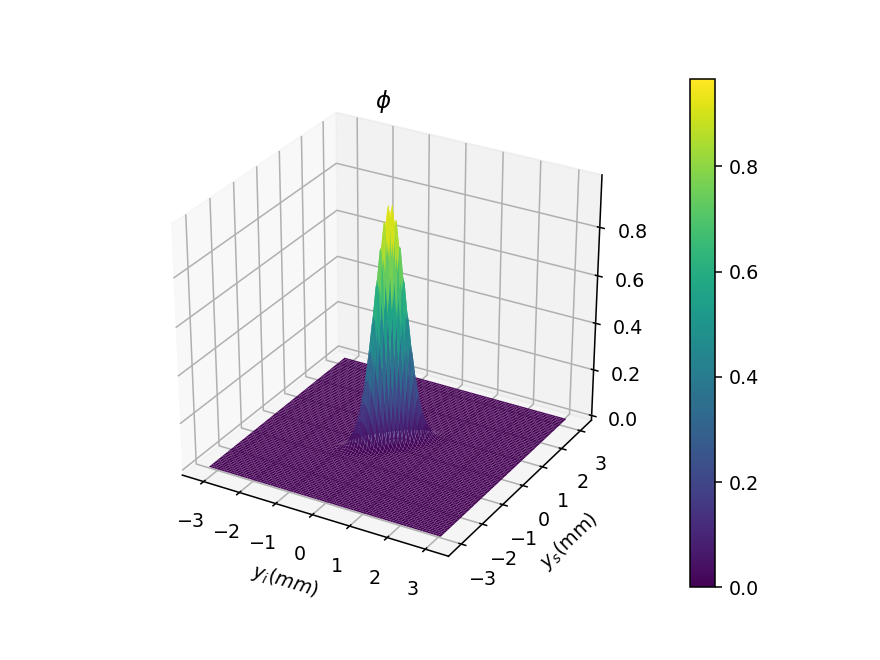
\includegraphics[width=\linewidth]{images/SPDC_yy.png}
\caption{YY correlation}
\end{subfigure}
\begin{subfigure}[b]{0.45\linewidth}
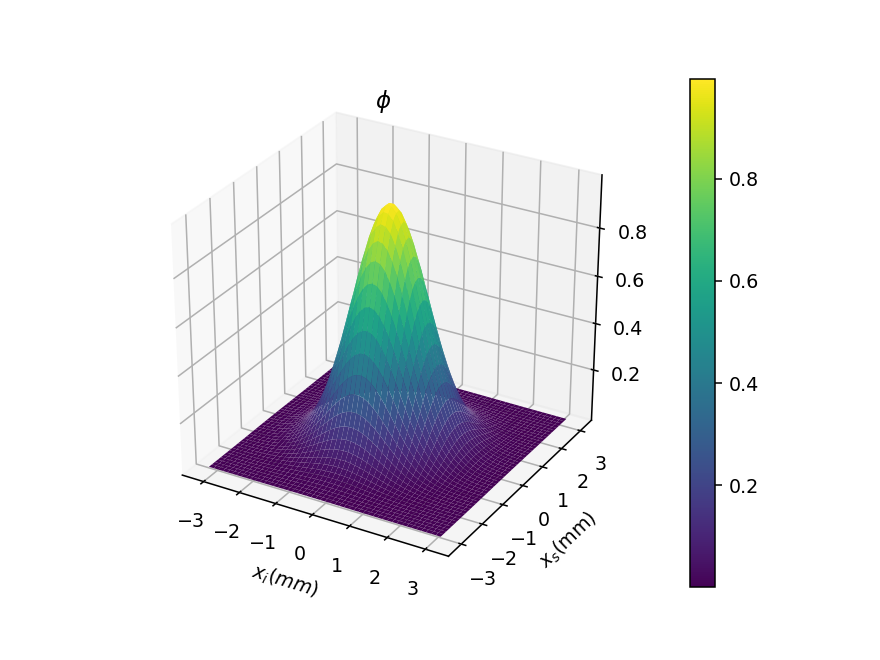
\includegraphics[width=\linewidth]{images/SPDC_xx.png}
\caption{XX correlation}
\end{subfigure}
\begin{subfigure}[b]{0.45\linewidth}
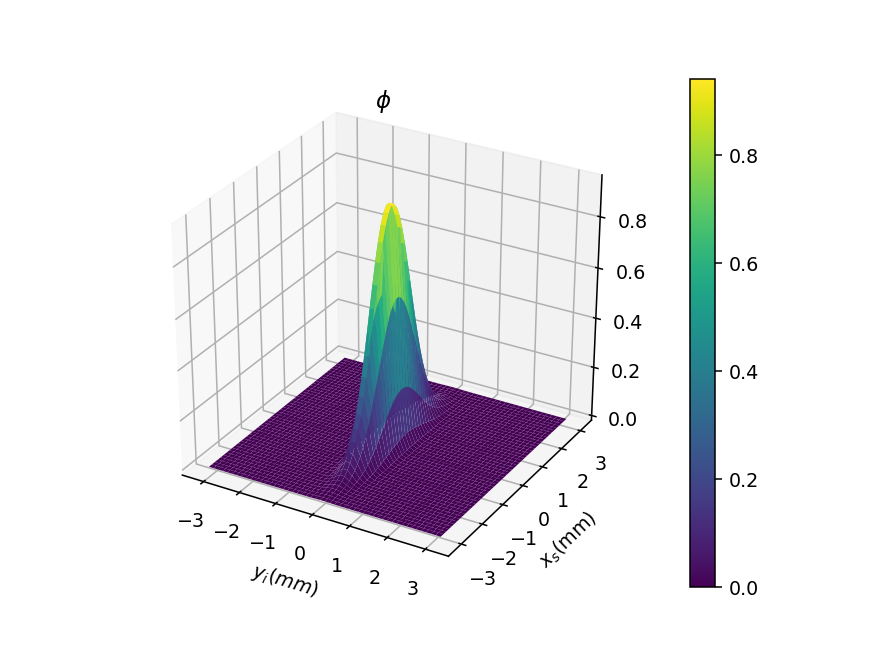
\includegraphics[width=\linewidth]{images/SPDC_yx.png}
\caption{YX correlation}
\end{subfigure}
\begin{subfigure}[b]{0.45\linewidth}
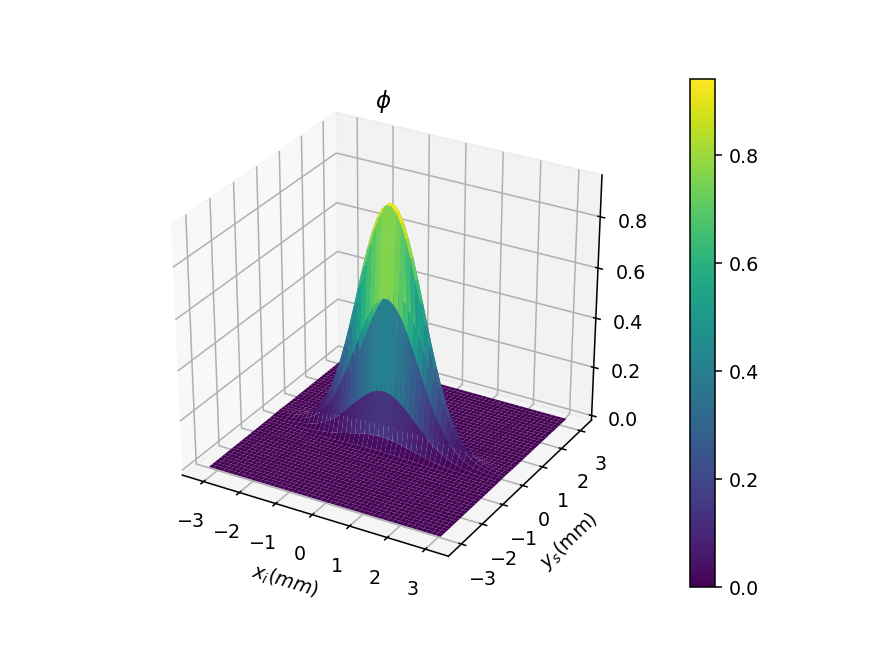
\includegraphics[width=\linewidth]{images/SPDC_xy.png}
\caption{XY correlation}
\end{subfigure}
\caption{Plots for $\Phi_{s}(x_{i},y_{i},x_{s},y_{s})$  from left to right are $x_{s}=x_{i}=0$ (a), $y_{s}=y_{i}=0$(b), $x_{i}=y_{s}=0$(c) and $y_{i}=x_{s}=0$(d). In all these plots we set $\sigma=0.18$, $\sigma_{x}=0.59$, $\sigma_{y}=0.1$.}
\label{SPDC}
\end{figure}


This last equation encodes all spatial correlations between the signal and idler photon channels, allowing us to use this scheme to study single-photon states, by measuring in two positions which are highly correlated and only taking into account measurements where both detectors (one placed in the signal channel and the other in the idler channel) click, ensuring that this process took place and we indeed have single-photon states.


\chapter{The lossless beam splitter}


In this chapter, we will develop both the classical and quantum theory of the most important optical element in this thesis, the beam splitter. The beam splitter is a four-port optical device with two inputs and two outputs, as shown in Fig. \ref{fig:BS}, in which two input beams may interfere to produce two outgoing beams. A beam splitter usually consists of two dielectric triangular prisms spliced in the form of a cube.

\section{The  classical lossless beam splitter}

This section is inspired in the beam splitter description presented in \cite{ludon} and \cite{leonhardt}. In this work, we will consider monochromatic light (one mode only) and we will assume that the beam splitter is an ideal reversible and lossless device.


In describing the behaviour of a laser beam in classical electrodynamics, it is common to consider the study of their corresponded electric fields, if the beams cross through a linear medium, the outgoing fields can be written as linear combinations of the input fields satisfying the proper boundary conditions \cite{jackson}. As in the beam splitter we have two inputs and two outputs, the output fields $E_{1}'$ and $E_{2}'$  can be written in terms of the input fields $E_{1}'$ and $E_{2}'$ as:

\begin{equation}
\begin{pmatrix} E_{1}' \\ E_{2}' \end{pmatrix}=B\begin{pmatrix} E_{1} \\ E_{2} \end{pmatrix},
\end{equation}

the linear transformation $B$ represents the action of the beam splitter on the input fields and is described by a matrix:

\begin{equation}
B=\begin{pmatrix} B_{11}& B_{12} \\B_{21} & B_{22} \end{pmatrix}.
\end{equation}

\begin{figure}[t!]
\centering
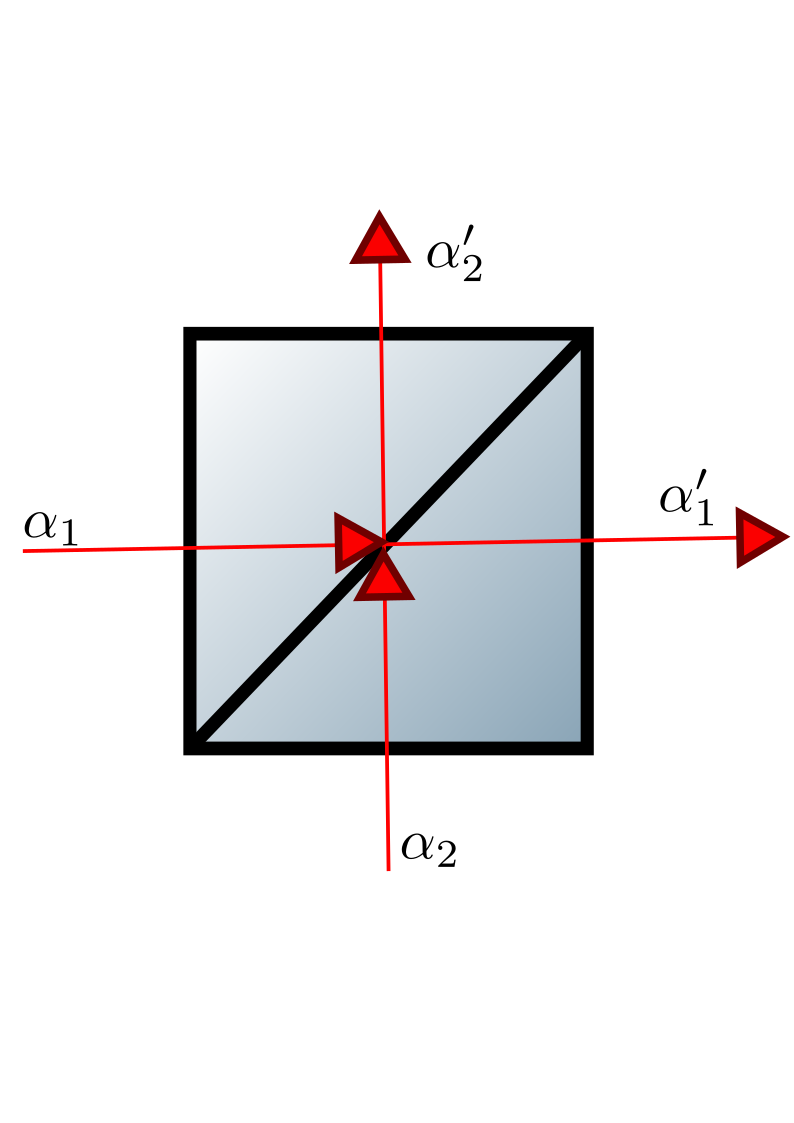
\includegraphics[width=5 cm,height=5 cm]{images/bS.png}
\caption{A Beam splitter cube.}
\label{fig:BS}
\end{figure}

The conditions  that must be fulfilled by the matrix elements $B_{ij}$  $i,j=1,2$  can be established by demanding the total intensity to be preserved (recall that we are considering that the beam splitter is a lossless device), that is:

\begin{align}
&I_{1}'+I_{2}'=I_{1}+I_{2}, \\
&I_{1}'\propto|B_{11} E_{1}|^{2}+|B_{12} E_{2}|^{2}+B_{11} B_{12}^{*} E_{1} E_{2}^{*}+B_{11}^{*} B_{12} E_{1}^{*} E_{2}, \\
&I_{2}'\propto|B_{21} E_{1}|^{2}+|B_{22} E_{2}|^{2}+B_{21} B_{22}^{*} E_{1} E_{2}^{*}+B_{21}^{*} B_{22} E_{1}^{*} E_{2},\\
&|E_{1}|^{2}+|E_{2}|^{2}=(|B_{21}|^{2}+|B_{11}|^{2})|E_{1}|^{2}+(|B_{12}|^{2}+|B_{22}|^{2})|E_{2}|^{2}\\
&+(B_{21} B_{22}^{*}+B_{11} B_{12}^{*})E_{1} E_{2}^{*}+(B_{21}^{*} B_{22}+B_{11}^{*} B_{12})E_{1}^{*} E_{2},
\end{align}

where $I_{1}$ and $I_{2}$ are the intensities of the input fields and $I_{1}'$ and $I_{2}'$ are the intensities of the output fields. Recall that the intensity of a given electric field is given by $I=\frac{c n \epsilon_{0}}{2} |E|^{2}$, where $c$ is the speed of light, $n$ the index of refraction of the medium and $\epsilon_{0}$ is the permitivity of free space, in this way the conservation of intensity (energy) leads us to the following relationships:

\begin{align}
&|B_{12}|^{2}+|B_{22}|^{2}=|B_{21}|^{2}+|B_{11}|^{2}=1,\\
&B_{21}^{*} B_{22}+B_{11}^{*} B_{12}=0.
\end{align}

These relations imply that the matrix $B$ is unitary. Yet, from this set of equations, one can derive another constraint on the coefficients, namely, $B_{21}^{*} B_{11}+B_{22}^{*} B_{12}=0$ can be obtained. This is consistent with the fact that $B^{\dagger}B=B^{\dagger}B= \mathbf{1}$. For our purposes it will be convenient to write the matrix $B$ in terms of the reflection $\rho$ and the transmission $\tau$, the transmission coefficient is a measure of how much light is transmitted through a material in relation to the amount of light incident on it, the reflection coefficient is a similar measure for reflection on the material. These coefficients follow the relationship:

\begin{equation}
|\tau|^{2}+|\rho|^{2}=1.
\end{equation}
 
 In the classical regime the transformation $B$ is usually written as:
 
 \begin{equation}
 B=\begin{pmatrix} \tau & \rho \\ -\rho & \tau \end{pmatrix},
 \end{equation}


so that

\begin{equation}
\begin{pmatrix} E_{1}' \\ E_{2}' \end{pmatrix}=\begin{pmatrix} \tau & \rho \\ -\rho & \tau \end{pmatrix} \begin{pmatrix} E_{1} \\ E_{2} \end{pmatrix}.
\end{equation}




\section{The quantum lossless beam splitter}

Now, we will describe the quantum theory of a lossless beam splitter. To do this we will first consider the quantized electric field and then we will establish the theory. 


The electric field of a polarized and monochromatic light beam can be written as:

\begin{equation}
\mathbf{E}=i \mathbf{\epsilon}N w \left( \alpha e^{i (\mathbf{k \cdot r}-w t)}+\alpha^{*} e^{-i (\mathbf{k \cdot r}-w t)} \right),
\end{equation}

where $\alpha$ is known as the complex wave amplitude. To obtain a theoretical model of a beam splitter as general as possible, let us describe the device as a four-port device, a black box with two input and two output ports.

If two coherent light beams with complex wave amplitudes $\alpha_{1}$ and $\alpha_{2}$ enter the beam splitter we simply expect the output complex wave amplitudes  are superimposed according to a linear transformation that we will call also $B$ as

\begin{equation}
\begin{pmatrix} \alpha_{1}' \\ \alpha_{2}' \end{pmatrix}=B\begin{pmatrix} \alpha_{1} \\ \alpha_{2} \end{pmatrix}. \label{ladilla}
\end{equation}

When the electric field  is quantized the complex wave amplitude $\alpha$ is promoted to a ladder operator \cite{ludon}. Once quantized the relation \ref{ladilla} becomes:

\begin{equation}
\begin{pmatrix} \mathbf{a}_{1}' \\ \mathbf{a}_{2}' \end{pmatrix}=B\begin{pmatrix} \mathbf{a}_{1} \\ \mathbf{a}_{2} \end{pmatrix}.
\label{eq:amplitudes}
\end{equation}

As this equation describes the transformation of the ladder operators in the process, it corresponds to the Heisenberg picture. Assuming the incoming and outgoing beams are both independent bosonic modes, we obtain some properties of the $B$ matrix as a consequence of the ladder operators commutation relationships:

\begin{align}
&[\mathbf{a}'_{\nu},\mathbf{a}'_{\mu}]=[\mathbf{a}_{\nu},\mathbf{a}_{\mu}]=0,\\
&[\mathbf{a}'_{\nu},\mathbf{a}'^{\dagger}_{\mu}]=[\mathbf{a}_{\nu},\mathbf{a}^{\dagger}_{\mu}]=\delta_{\mu \nu},
\label{commutators}
\end{align}

where $\mu=1,2$ and $\nu=1,2$. From Eq. \ref{eq:amplitudes} it follows that:

\begin{align}
&\mathbf{a}'_{\mu}=B_{\mu 1}\mathbf{a}_{1}+B_{\mu 2} \mathbf{a}_{2}, \\
&\mathbf{a}'^{\dagger}_{\mu}=B_{\mu 1}^{*}\mathbf{a}^{\dagger}_{1}+B_{\mu 2}^{*} \mathbf{a}^{\dagger}_{2}.
\label{combined amplitudes}
\end{align}

Then using Eq. \ref{combined amplitudes} and Eq. \ref{commutators} we find 

\begin{equation}
   [\mathbf{a}'_{\nu},\mathbf{a}'^{\dagger}_{\mu}]=B_{\nu 1} B_{\mu 1}^{*}+B_{\nu 2} B_{\mu 2}^{*} .
\end{equation}

Substituting all the possible values of $\nu$ and $\mu$ we find the following relationships:

\begin{equation}
|B_{11}|^{2}+|B_{12}|^{2}=|B_{21}|^{2}+|B_{22}|^{2}=1 ,\qquad B_{11} B_{21}^{*}+B_{12} B_{22}^{*}=0.
\end{equation}

As in the classical case, we find the $B$ transformation to be unitary, something expected as the beam splitter is still a lossless device. The most general form of a unitary $2\times2$ matrix is \cite{leonhardt}:


\begin{equation}
B=e^{\Lambda} \begin{pmatrix} e^{i\frac{\phi}{2}} & 0 \\ 0 & e^{-i\frac{\phi}{2}} \end{pmatrix} \begin{pmatrix} \cos(\theta) &  \sin(\theta) \\ - \sin(\theta) & \cos(\theta) \end{pmatrix} \begin{pmatrix} e^{i\frac{\psi}{2}} & 0 \\ 0 & e^{-i\frac{\psi}{2}} \end{pmatrix} \label{unitary},
\end{equation}

where $\psi,\Lambda,\theta,\phi$ are real parameters in the interval $[0,2\pi)$. Note that so far our analysis is valid for any linear and lossless four-port device. Furthermore, from Eq. \ref{unitary} we can see that any four-port device can be considered as acting in three steps \footnote{A phase shifter is denoted by $P_{\phi}=e^{i \frac{\phi}{2}}\begin{pmatrix}e^{i \frac{\phi}{2}} & 0 \\0 & e^{-i \frac{\phi}{2}} \end{pmatrix}$}. First, the phases of the incident modes are changed, then the amplitudes are mixed (rotated) and then the phases are changed again. In most cases we can adjust the reference phases such that only the rotation is important (a reference phase is the phase from which we start measuring phase-shifts), so this is the key feature of four-ports, that is why from now on we will parametrize our beam splitter ($BS$) as (this corresponds to  setting $\Lambda=0$, $\phi=-\psi=\frac{\pi}{2}$):


\begin{equation}
BS=\begin{pmatrix} \cos(\theta) & i \sin(\theta) \\ i \sin(\theta) & \cos(\theta) \end{pmatrix}.\label{BS_matrix}
\end{equation}


The difference between $B$ and $BS$ is that $B$ is general and in $BS$ we fixed the parameters that involve phase-shifting and the global phase. Let us now analyze this optical element in the Fock basis  to use it on a single-photon state. In the Heisenberg picture operators evolve via the evolution operator:

\begin{equation}
\begin{pmatrix} \mathbf{a}'_{1} \\ \mathbf{a}'_{2}\end{pmatrix}=\mathbf{U}^{\dagger}_{B} \begin{pmatrix} \mathbf{a}_{1} \\ \mathbf{a}_{2}\end{pmatrix} \mathbf{U}_{B}.
\label{Heisenberg}
\end{equation}

A Fock state $\ket{n_{1},n_{2}}$, which means $n_{1}$ photons in the first input(output) and $n_{2}$ photons in the second input(output), can be generated from a vacuum state through the subsequent application on creation operators  $\mathbf{a}^{\dagger}_{1}\mathbf{a}^{\dagger}_{2}$. 

\begin{equation}
 \ket{n_{1},n_{2}}=\frac{1}{\sqrt{n_{1}! n_{2}!}} (\mathbf{a}_{1}^{\dagger})^{n_{1}}(\mathbf{a}_{2}^{\dagger})^{n_{2}} \ket{0,0}.
\end{equation}

Note that if just one of the input channels is pumped, then the state corresponding to the other one is a vacuum state $\ket{0}$. Correspondingly, in the Schrodinger picture a state $\ket{\psi}$ evolves by means of the rule:

\begin{equation}
 \ket{\psi}'=U_{B}\ket{\psi},
\end{equation}

so for the vacuum state we have:
\begin{equation}
 \ket{0,0}'=U_{B}\ket{0,0}.
 \label{evolution}
\end{equation}

The evolution of a Fock state $\ket{n_{1},n_{2}}'$:

\begin{align}
&\ket{n_{1},n_{2}}'=U_{B}\ket{n_{1},n_{2}},\\
&\ket{n_{1},n_{2}}'=\frac{U_{B}}{\sqrt{n_{1}! n_{2}!}} (\mathbf{a}_{1}'^{\dagger})^{n_{1}}(\mathbf{a}_{2}'^{\dagger})^{n_{2}} \ket{0,0}.
\end{align}

From Eq. \ref{Heisenberg}, Eq. \ref{eq:amplitudes} and Eq. \ref{evolution} we can obtain:

\begin{align}
&\ket{n_{1},n_{2}}' =\frac{U_{B}}{\sqrt{n_{1}! n_{2}!}} (\mathbf{a}_{1}'^{\dagger})^{n_{1}}(\mathbf{a}_{2}'^{\dagger})^{n_{2}} U^{\dagger}_{B}\ket{0,0}',\\
&\ket{n_{1},n_{2}}' =\frac{1}{\sqrt{n_{1}! n_{2}!}} (\mathbf{a}_{1}^{\dagger})^{n_{1}}(\mathbf{a}_{2}^{\dagger})^{n_{2}}\ket{0,0}'.
\end{align}

By writing the original ladder operators in terms of the transformed ladder operators given by Eq. \ref{eq:amplitudes}, and applying Newton's binomial formula (we can do this because the operators commute, in general this cannot be done) we arrive at the expression \footnote{ The binomial coefficient is $\begin{pmatrix} n \\ k \end{pmatrix} =\frac{n!}{\sqrt{k!(n-k)!}}$}:

\begin{align*}
\ket{n_{1},n_{2}}'& =\frac{1}{\sqrt{n_{1}! n_{2}!}} (B_{11}\mathbf{a}_{1}'^{\dagger}+B_{21}\mathbf{a}_{2}'^{\dagger})^{n_{1}}(B_{12}\mathbf{a}_{1}'^{\dagger}+B_{22}\mathbf{a}_{2}'^{\dagger})^{n_{2}}\ket{0,0}',\\
\ket{n_{1},n_{2}}'&=\frac{1}{\sqrt{n_{1}! n_{2}!}}\sum^{n_{1},n_{2}}_{k_{1},k_{2}=0}\begin{pmatrix} n_{1} \\ k_{1} \end{pmatrix}\begin{pmatrix} n_{2} \\ k_{2} \end{pmatrix} B_{11}^{n_{1}-k_{1}} B_{21}^{k_{1}} B_{12}^{n_{2}-k_{2}} B_{22}^{k_{2}} \\
\times &\sqrt{(n_{1}+n_{2}-k_{1}-k_{2})!(k_{1}+k_{2})!} \ket{n_{1}+n_{2}-k_{1}-k_{2},k_{1}+k_{2}}' .\numberthis{}
\end{align*}

Now let us consider in one of the inputs we have a vacuum state that is, $n_{2}=0$ and $n_{1}=n$  and vice-versa (from now on we will drop the primes on the right hand side):
\begin{equation}
 \ket{n,0}'=\sum^{n}_{k=0} \sqrt{\frac{n!}{(n-k)!k!}} B_{11}^{n-k} B_{21}^{k} \ket{n-k,k}
\end{equation}
and its counterpart
\begin{equation}
     \ket{0,n}'=\sum^{n}_{k=0} \sqrt{\frac{n!}{(n-k)!k!}} B_{12}^{n-k} B_{22}^{k} \ket{n-k,k}.
\end{equation}

In this work will consider single-photons states in the input channels, so that our case of interest is $n=1$,we expand the sum to obtain:

\begin{align}
\ket{1,0}'=B_{11}\ket{1,0}+B_{21}\ket{0,1},\label{basis2} \\
\ket{0,1}'=B_{12}\ket{1,0}+B_{22}\ket{0,1}.
\label{basis}
\end{align}


From Eqs. \ref{basis2}-\ref{basis}, we can see that the evolution of a single-photon state can be written in terms of the $BS$ matrix if we define an appropriate basis to describe the system. The one we will use is the Horizontal-Vertical computational basis. We will use:

 \begin{equation}
 \ket{1}=\ket{1}_{h}\ket{0}_{v}=\begin{pmatrix} 1 \\0\end{pmatrix},
 \end{equation}

 meaning one photon in the horizontal path and vacuum in the vertical one, and
 
 \begin{equation}
 \ket{2}=\ket{0}_{h}\ket{1}_{v}=\begin{pmatrix} 0 \\1 \end{pmatrix},
 \end{equation}
 
meaning vacuum  in the horizontal path and one photon in the vertical one. In this terms Eq. \ref{basis} becomes:

\begin{equation}
\ket{out}=\begin{pmatrix} \cos(\theta) & i \sin(\theta) \\ i \sin(\theta) & \cos(\theta) \end{pmatrix} \ket{in},
\end{equation}

where $\ket{in}=\ket{1},\ket{2}$ and out is a linear combination of the vectors $\ket{1},\ket{2}$.

 It should not be a surprise that we obtain a similar description of the beam splitter in the classical and quantum theories. Typically, classical and quantum interference phenomena differ in the visibility of the effect and not in the final mathematical predictions \cite{leonhardt}.

\pagebreak

\chapter{The Mach-Zehnder interferometer }


 The Mach–Zehnder's flexibility in locating fringes in interference patterns has made it the preferred interferometer for visualizing flow in wind tunnels \cite{10} and for flow visualization studies in general. It is frequently used in several fields such as aerodynamics, plasma physics, and heat transfer to measure pressure, density, and temperature changes in gases \cite{11}. They are also used in electro-optic modulators \cite{ackerman} and electronic devices used in various fiber-optic communication applications. Mach–Zehnder modulators are incorporated in monolithic integrated circuits and offer well-behaved, high-bandwidth electro-optic amplitude, and phase responses over a multiple-gigahertz frequency range \cite{studenkov,capmany}.

The Mach-Zehnder interferometer consists of two Beam Splitters, $BS_{1}$ and $BS_{2}$, and two mirrors $M_{1}$ and $M_{2}$ as shown, in Fig. \ref{fig:classical mach}. One of the input channels of the first beam splitter $BS_{1}$ is pumped by a light beam to produce two output signals that are redirected by the two mirrors $M_{1}$ and $M_{2}$ towards the input ports of the second $BS_{2}$.  Two detectors $D_{1}$ and $D_{2}$ placed at the output ports will  sense the interference pattern of the recombined beams $E_{1}'''$ and $E_{2}'''$. We will now analyze the interferometer, both, in the classical and quantum regimes.


 A mirror in this basis (Horizontal-Vertical) simply flips the state and adds a phase, so we have no recombination of the amplitudes (which corresponds to no rotations only phase shifting) taking Eq. \ref{unitary} with $\theta=\frac{\pi}{2}$, $\phi=\pi$, $\Lambda=\gamma$ and $\psi= \frac{\pi}{2} $ we obtain the matrix $M$ representing a mirror:

 
\begin{equation}
M=\begin{pmatrix} 0& e^{i\gamma}  \\ e^{i\gamma} & 0 \end{pmatrix}, \label{mirror}
\end{equation}


 We have now defined all the elements of the interferometer in the classical and quantum regimes.

\begin{figure}[H]
\centering
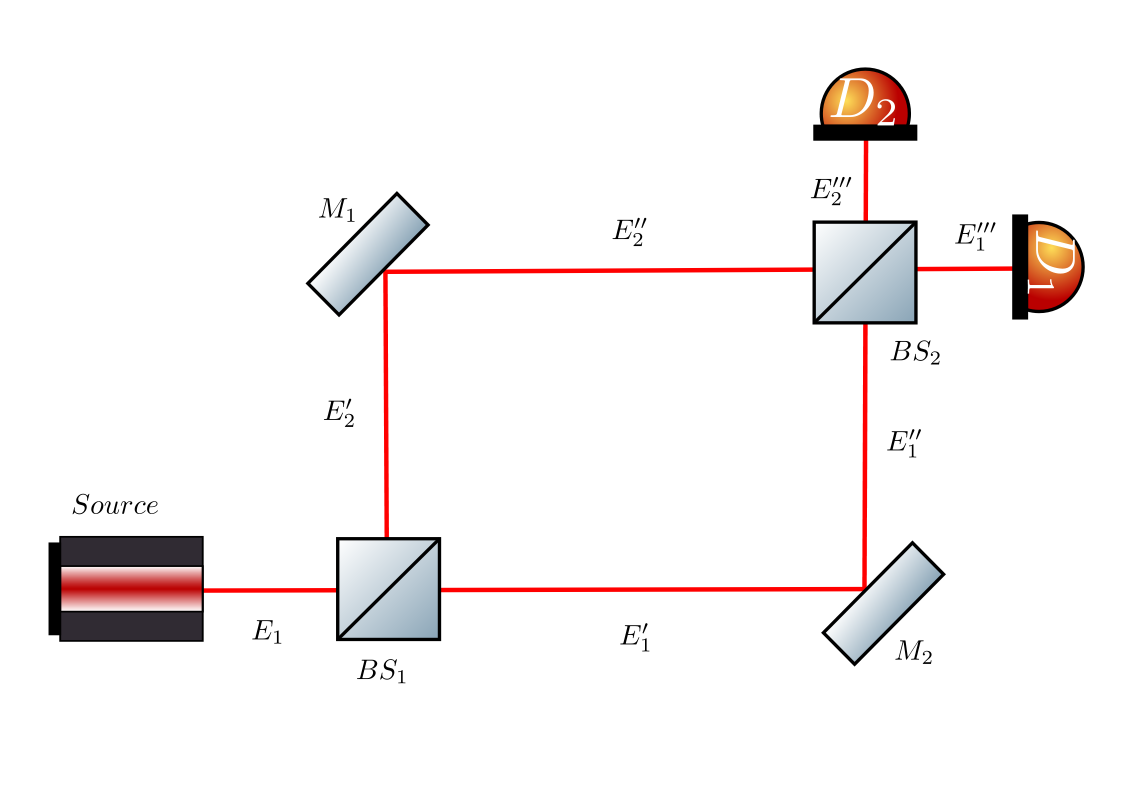
\includegraphics[width=\linewidth]{images/machzenhdercla.png}
\caption{Mach-Zehnder interferometer.}
\label{fig:classical mach}
\end{figure}



\section{Classical Mach-Zehnder interferometer}

In this section, we study the Mach-Zehnder interferometer in the classical regime. We will denote the classical fields going through the interferometer as it is shown in Fig. \ref{fig:classical mach}. We will follow the approach taken by Loudon \cite{ludon}. Let us consider two lossless beam splitters   $BS_{1}$, $BS_{2}$ with the same reflectivity $\rho$ and transmitivity $\tau$. After the first beam splitter, the electric field $E_{1}$ of the incident beam is split into two beams $E_{1}'$ and $E_{2}'$ written as:

\begin{equation}
E_{1}'=\tau E_{1} ,\qquad E_{2}'=\rho E_{1}.\label{corr1}
\end{equation}

The action of the matrix $M$ representing the mirrors only add a phase $e^{i\gamma_{i}}$, where $i=1,2$. As a second stage, after the light strikes the mirrors $M_{1}$ and $M_{2}$, the electric fields $E_{1}''$ and $E_{2}''$ in each path are:

\begin{equation}
 E_{1}''=e^{i\gamma_{1}}E_{1}', \qquad E_{2}''=e^{i \gamma_{2}}E_{2}'.\label{corr2}
\end{equation}

As a final stage, the fields are recombined in the second beam splitter $BS_{2}$ producing the output fields $E_{1}'''$ and $E_{2}'''$:

\begin{align*}
E_{1}'''=\tau E_{2}'' +\rho E_{1}'', \qquad E_{2}'''=\tau E_{1}'' -\rho E_{2}''.\label{corr} \numberthis
\end{align*}

We can write the output in terms of the input field substituting Eqs. \ref{corr1}, \ref{corr2} in Eq. \ref{corr} as :

\begin{align*}
E_{1}'''&=\tau \rho (e^{i \gamma_{1}}+ e^{i \gamma_{2}})E_{1},\\
E_{2}'''&=(\tau^2 e^{i \gamma_{1}}  -\rho^2 e^{i \gamma_{2}})E_{1}.
 \numberthis
\end{align*}

The intensities at the detectors can be calculated by taking the modulus squared of the fields, where $\delta \gamma=\gamma_{1}-\gamma_{2}$:

\begin{align*}
I_{D_{1}}& \propto \abs{E_{1}}^2 2 |\rho \tau|^2\left[1+\cos(\delta \phi)\right],\\
I_{D_{2}}& \propto \abs{E_{1}}^2 (|\rho|^4 +|\tau|^4)\left[1-\frac{2 |\rho \tau|^2}{|\rho|^4+|\tau|^4}\cos(\delta \phi)\right]. \numberthis
\end{align*}

A case of interest occurs whenever $\rho =\tau=\frac{1}{\sqrt{2}}$. In this circumstances the intensities become:

\begin{align*}
I_{D_{1}}  \propto \abs{E_{1}}^2 \frac{1+\cos(\delta \phi)}{2}, \quad
I_{D_{2}}  \propto \abs{E_{1}}^2 \frac{1-\cos(\delta \phi)}{2}. \numberthis
\end{align*}
 
 If additionally   $\delta \gamma=2 \pi n$ where $n=1,2,3,...$, then $\cos(2 \pi n )=1$ and the detector $D_{1}$ receives the intensity of the initial beam $I_{D_{1}}\propto \abs{E_{1}}^2$ and $D_{2}$ receives no light $I_{D_{2}}= 0.$


\section{Single-photon Mach-Zehnder interferometer}

In this section, we will study a single-photon Mach-Zehnder interferometer, which will be the main object of concern for the rest of this work. In this part of the analysis, we will assume that the mirrors induce different phases in each path. This is done to account for misalignment in our model. It will be proven in a later chapter that this is equivalent to considering phase-shifters inducing differences in the optical paths. We write the matrix representation of the mirrors as:

\begin{equation}
M_{i}= \begin{pmatrix} 0& e^{i\gamma_{i}} \\ e^{i\gamma_{i}} & 0 \end{pmatrix}, \quad i=1,2.
\end{equation}

and a beam splitter as in Eq. \ref{BS_matrix}. Once we have defined the main elements we can analyze the single-photon Mach-Zehnder interferometer. A single photon, generated via SPDC, is sent into the horizontal path of the interferometer as the input signal. In order to study a general situation, we will consider two different $BS$ in our interferometer. Then, our initial state $\ket{1}$  is transformed by the first $BS$ as:

\begin{align}
\ket{1}\xrightarrow{\text{BS1}}\cos(\theta_{1})\ket{1}+i\sin(\theta_{1})\ket{2}.
\numberthis
\end{align}

 Note that the action of optical elements is local, meaning that the matrix $M_1$ ($M_2$) acts only onto the input state of the mirror$\ket{2}$ ($\ket{1}$). After passing through the first $BS$, the photon encounters a mirror in each path, and then both paths are recombined in the second $BS$, as in Fig. \ref{fig:classical mach}. The whole action of the interferometer on the initial state $\ket{1}$ is then:


\begin{align*}
&\ket{1}\xrightarrow{\text{BS1}}\cos(\theta_{1})\ket{1}+i\sin(\theta_{1})\ket{2}\xrightarrow{\text{Mirrors}}\cos(\theta_{1})e^{i\gamma_{1}}\ket{2}+i\sin(\theta_{1})e^{i\gamma_{2}}\ket{1} \\ \xrightarrow{\text{BS2}}
 &i\left[\cos(\theta_{1})\sin(\theta_{2})e^{i\gamma_{1}}+\cos(\theta_{2})\sin(\theta_{1})e^{i\gamma_{2}}\right]\ket{1}+\\&\left[\cos(\theta_{1})\cos(\theta_{2})e^{i\gamma_{1}}-\sin(\theta_{1})\sin(\theta_{2})e^{i\gamma_{2}}\right]\ket{2}. \numberthis
\end{align*}


To compare this result with the classical case for which we consider two identical $BS$, we make $\theta_{1}=\theta_{2}=\frac{\pi}{4}$. Then the state $\ket{\psi}$ at the output of the interferometer is

\begin{align*}
\ket{\psi}&=\frac{i}{2}(e^{i\gamma_{1}}+e^{i\gamma_{2}})\ket{1}+\frac{1}{2}(e^{i\gamma_{1}}-e^{i\gamma_{2}})\ket{2}, \\
&=\frac{e^{i(\gamma_{1}+\frac{\pi}{2})}}{2}(1+e^{i(\gamma_{2}-\gamma_{1})})\ket{1}+\frac{e^{i\gamma_{1}}}{2}(1-e^{i(\gamma_{2}-\gamma_{1})})\ket{2}. \numberthis
\end{align*}

To obtain the probabilities of detection, we simply compute:
\begin{align}
P_{D_{1}}&=|\bra{1}\ket{\psi}|^{2}, \qquad &&P_{D_{2}}=|\bra{2}\ket{\psi}|^{2},\\
P_{D_{1}}&=\frac{1+\cos(\gamma_{2}-\gamma_{1})}{2}, \qquad &&P_{D_{2}}=\frac{1-\cos(\gamma_{2}-\gamma_{1})}{2}. \label{pp_wheler}
\end{align}

Perfect alignment means no difference in the optical path so that $\gamma_{2}-\gamma_{1}=0$, then the probability to detect a photon in $D_{1}$ is one and in $D_{2}$ is zero, perfectly compatible with the result obtained in the classical case. We expect a similar result because the classical case is nothing but many repetitions of the single-photon phenomenom.

\section[Analysis with phase retarders]{Analysis of a Mach-Zhender interferometer with additional phase retarders}

The interferometer is an instrument quite hard to align experimentally, in most cases alignment is a little off. We can characterize just how off this alignment is by considering the effects of phase retarders on each arm of the interferometer, after all misalignment is nothing but differences in the optical path. Those predictions can be compared with the actual interferometer (without phase retarders), a wave retarder's  matrix representation is :


\begin{equation}
 R=\begin
{pmatrix} e^
{i c} & 0\\0& e^
{i k }\end
{pmatrix},
\end{equation}

when placed in the horizontal path $k=0$ and when placed in the vertical $c=0$. Let us see the effect of such an optical device in our setup:

\begin{align*}
&\ket{1}\xrightarrow{\text{BS1}}\cos(\theta_{1})\ket{1}+i\sin(\theta_{1})\ket{2}\\ &\xrightarrow[\text{Retarders}]{\text{Phase}}\cos(\theta_{1})e^{ic}\ket{1}+i\sin(\theta_{1}) e^{ik}\ket{2} \\ &\xrightarrow{\text{Mirrors}} \cos(\theta_{1})e^{i(\frac{\pi}{2}+c)}\ket{2}+i\sin(\theta_{1})\beta e^{i(\frac{\pi}{2}+k)}\ket{1},
\end{align*}

we can stop here by noticing that replacing $\frac{\pi}{2}+k\xrightarrow{}\gamma_{2}$ and  $\frac{\pi}{2}+c\xrightarrow{}\gamma_{1}$, is the same as using the mirror matrix given by Eq. \ref{mirror} so our model that makes use of this matrix  instead of the more popular mirror matrix with a fixed phase $M=\begin{pmatrix} i & 0\\0& i\end{pmatrix}$, where $i=e^{i \frac{\pi}{2}}=e^{i\gamma}$, has the  effect of a phase retarder included, allowing us to study misalignment. 

\afterpage{\blankpage}

\chapter[Interaction-free measurements]{ Interaction-free  measurements}


In this chapter, we will explore what is known in the literature as interaction-free measurements. The possibility of performing such kind of measurements was first reported by Elitzur and Vaidman in \cite{Elitzur}. Since then, the topic has awakened a lot of discussion about the non-local nature of quantum theory as well as the philosophical interpretations of quantum mechanics\footnote{ This philosophical discussions will be kept to a minimum in this thesis since they are way more philosophical than physical and highly speculative. Interesting discussions can be found in \cite{paper_vaidman, maudlin}. }. We will now analyze the simplest case proposed by Elitzur and Vaidman

\section[Elitzur-Vaidman's bomb detector]{Single-photon Mach-Zehnder interferometer with a perfect absorber}

Consider a Mach-Zehnder interferometer where we could or could not place  a perfectly absorbent object in one of its paths. Consider also that a single photon is traveling through the interferometer. This system is best known as the Elitzur-Vaidman's bomb detector \cite{Elitzur}. In order to express their ideas in a more dramatic way, Elitzurt and Vaidman proposed that the perfect absorber may be a bomb that is sensitive to the interaction with a single-photon. The bomb is supposed to explode if only a single-photon enters its sensor. An interesting aspect of this experiment is that it exhibits the non-local nature of quantum mechanics, as it allows the possibility of getting knowledge of whether the perfect absorber is in one of the arms of the interferometer performing a measurement without touching it. Yet, Elitzur and Vaidman showed that the single-photon Mach-Zehnder interferometer supplies a mechanism to detect if the bomb was there, without exploding it. They concluded that this can be achieved in, at most, $25\%$ the events.


\begin{figure}[t!]
\centering
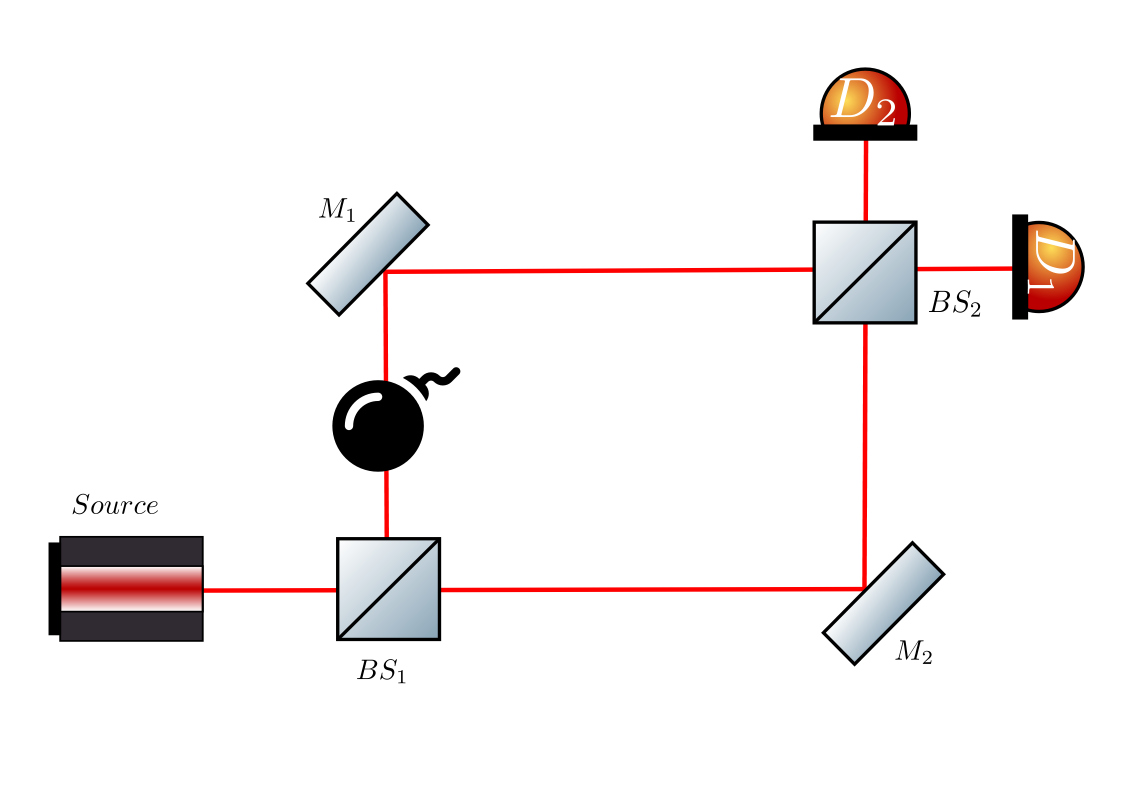
\includegraphics[width=\linewidth]{images/machzenhderbomb.png}
\caption{Elitzur-Vaidman's bomb detector.}
\label{fig:bomb}
\end{figure}

To analyze this system, we will consider the Mach-Zehnder model of section 3.2 but this time having a perfect absorber in its vertical arm, as Fig. \ref{fig:bomb} shows. We will also consider that once the photon is absorbed, the optical elements of the interferometer do not interact with it any longer. We will denote the state corresponding to an absorbed photon by means of the $\ket{abs}$ vector. Assume a single-photon is pumped in the horizontal input channel of the Mach-Zehnder interferometer. First, the initial state of the system is transformed by the beam splitter $BS_{1}$, into a superposition state of the single photon being transmitted to the horizontal output of $BS_{1}$ and being reflected to the vertical one. Then, the photon could either be absorbed by the bomb if it was traveling towards $M_1$ or be reflected by $M_2$ if it was traveling in the other arm. The mirror $M_{2}$, in turn, transforms the state into the state of the photon being redirected to the beam splitter $BS_{2}$, where it is finally split into the linear combination of being transmitted to detector $D_{2}$ or reflected to detector $D_{1}$. We have 
 
\begin{align*}
&\ket{1}\xrightarrow{\text{BS1}}\cos(\theta_{1})\ket{1}+i\sin(\theta_{1})\ket{2}\\ &\xrightarrow{\text{Bomb}}\cos(\theta_{1})\ket{1}+i\sin(\theta_{1})\ket{abs}\\ &\xrightarrow{\text{Mirrors}}
 i\cos(\theta_{1})\ket{2}+i\sin(\theta_{1})\ket{abs} \\ &\xrightarrow{\text{BS2}}i\cos(\theta_{1})\cos(\theta_{2})\ket{2}-\cos(\theta_{1})\sin(\theta_{2})\ket{1}+i\sin(\theta_{1})\ket{abs}, \numberthis
\end{align*}

where $M_{2}$ is such that $\gamma=\frac{\pi}{2}$, and $\theta_{1},\theta_{2}$ are the parameters in the beam splitter matrix for $BS_{1},BS_{2}$. The probabilities to be either absorbed or detected at either $D_{1}$ or $D_{2}$ are given by:

\begin{equation}
P_{D_{1}}=\cos^2(\theta_{1}) \sin^2(\theta_{2}),\qquad P_{D_{2}}=\cos^2(\theta_{1}) \cos^2(\theta_{2}),\qquad P_{abs}=\sin^2(\theta_{1}).
\end{equation}

As a particular case, if both, $BS_{1}$ and $BS_{2}$ are $50:50$ beam splitters, i.e where $\theta_{1}=\theta_{2}=\frac{\pi}{4}$, then:

\begin{equation}
P_{D_{1}}=\frac{1}{4},\quad P_{D_{2}}=\frac{1}{4}, \quad P_{abs}=\frac{1}{2}.
\end{equation}



If we detect the photon in $D_{1}$, we get no useful information to conclude about the presence of the bomb, as this result is always obtained in the conventional Mach-Zehnder interferometer. Thus, in $\frac{1}{2}$ of the times we make a measurement we cannot tell whether the bomb is there or not. In this experiment, the bomb has a $\frac{1}{2}$ probability of exploding by interacting with the photon. Additionally there is a $\frac{1}{2}$ probability that the photon is detected either at $D_{1}$ or $D_{2}$. So fifty percent of the time we have interaction-free measurements, to tell whether an object is there or not we need to consider that if the photon is detected at $D_{2}$, then it indicates that there is an object in one of the arms of the interferometer. However, we cannot distinguish between this case and the previous one section 3.2 from a single event if we detect at $D_{1}$, so $\frac{1}{2}$ of the times we make a measurement we can't tell if a bomb is there or not. Since we are dealing with just one measurement it is not so useful to talk about conditional probabilities such as, 'what is the probability of detecting in $D_{2}$, if the object is not absorbed' in the same way that it is not useful to talk about the probability of having a single dice throw come out as six provided it was not one. However, it is useful to analyze the efficiency of this interferometer, that is just how probable it is for us to realize interaction-free measurements, the efficiency is given by \cite{5}:

\begin{equation}
\eta=\frac{P_{det}}{P_{det}+P_{abs}},
\end{equation}

where $\eta$ is the efficiency, $P_{det}$ is the probability the object is detected, considering lossless optical devices, which we do in this work $P_{det}+P_{abs}=1$ and we have

\begin{equation}
\eta=P_{D_{1}}+P_{D_{2}}.
\end{equation}

For example in the case we explored in this section $\eta=\frac{1}{2}$.  Whenever a perfect absorber is in one of the arms of the interferometer, detecting a photon in either $D_1$ or $D_2$ means that the photon did not interacted with the bomb. As discussed above, detecting at $D_1$ does not give us information about the presence of the bomb. Since the goal is to determine if the bomb is there, a detection in $D_2$ is an ‘interaction-free measurement’ that confirms the presence of the bomb.
  
\section[Replacing the bomb with an imperfect transmitter]{Replacing the bomb with an imperfect transmitter}

This section is based on the treatment reported by Z. Blanco-Garcia and O. Rosas-Ortiz \cite{zuri,azuri}, and the work by Azuma \cite{Azuma}. 


Let us replace the ``bomb'' from section 4.1 with a semi-transparent object. The absorption and transmission coefficients of such an object will be denoted by $\alpha$ and $\beta$ , respectively, satisfying the condition $|\alpha|^2 + |\beta|^2 = 1.$



In the same Horizontal-Vertical basis, our initial state is $\ket{1}$. We will place our imperfect transmitter in the vertical output path of the beam splitter $BS_{1}$ as Fig. \ref{fig:bomb} shows. Our transmitter can either transmit with probability $|\beta|^2$ or absorb with probability $|\alpha|^2$, when a photon in the state $\ket{2}$ travels throught the object, the state transforms as:


\begin{align}
\ket{2}\xrightarrow[\text{Absorber}]{\text{Imperfect}}\alpha \ket{abs} +\beta \ket{2}.
\end{align}

With this information model the experiment. We start out with a photon state at the horizontal entry port of $BS_1$. Then, the initial state is transformed by $BS_{1}$ into a superposition of $\ket{1}$ and $\ket{2}$. The vertical component interacts with the so called by the imperfect transmitter which decomposes the component $\ket{2}$ into a superposition of $\ket{2}$ and $\ket{abs}$ (being transmited or being absorbed). Afterwards, the mirror in each path interchanges $\ket{1}\rightarrow{}\ket{2}$ and vice versa, in this section we will consider mirrors such that $\gamma=\frac{\pi}{2}$. Finally, the state is recombined in the second beam splitter $BS_{2}$. Mathematically, this process is written as 

\begin{align*}
& \ket{1}\xrightarrow{\text{BS1}}\cos(\theta_{1})\ket{1}+i\sin(\theta_{1})\ket{2} \\ &\xrightarrow[\text{Absorber}]{\text{Imperfect }}\cos(\theta_{1})\ket{1}+i\sin(\theta_{1})(\alpha \ket{abs} +\beta \ket{2} )
\\ &\xrightarrow{\text{Mirrors}} i\cos(\theta_{1})\ket{2}+i \sin(\theta_{1})\alpha\ket{abs}-\sin(\theta_{1})\beta\ket{1} \\ &\xrightarrow{\text{BS2}} -
(\cos(\theta_{1})\sin(\theta_{2})+\beta \sin(\theta_{1})\cos(\theta_{2}))\ket{1}+ i \alpha \sin(\theta_{1})\ket{abs} \\ &+i(\cos(\theta_{1})\cos(\theta_{2})-\sin(\theta_{1})\sin(\theta_{2})\beta)\ket{2}. \numberthis
\end{align*}

Then, the probabilities of detection at $D_1$, $D_2$ and absorption of the photon are 
\begin{align}
& P_{D_{1}}=|\cos(\theta_{1})\sin(\theta_{2})+\beta \sin(\theta_{1})\cos(\theta_{2})|^2, \label{eq1}\\
& P_{D_{2}}=|\cos(\theta_{1})\cos(\theta_{2})-\beta \sin(\theta_{1})\sin(\theta_{2})|^2, \\
& P_{abs}=|\alpha \sin(\theta_{1})|^2. \label{eq2}
\end{align}

Again, detection at $D_1$ tell us nothing about the presence of the object. But if we detect at $D_2$ we know that the object was in the vertical arm of the interferometer. Some people argue that this is no longer an interaction-free measurement because the photon may have passed through  the semitransparent object, they refer to this kind of setup as 'quantum interrogation' \cite{QI1,QI2}. 


From, now on we will write detection probabilities as $P_{ij}$ where $i=1$ ($i=2$) means that the object was placed just after $BS_1$ in the horizontal (vertical) arm of the interferometer, in previous calculation $i=2$. Subindex $j$ denotes one of the possible outcomes $j=D_{1},D_{2},abs$. In this notation $P_{D_1}= P_{2D_{1}}, ~P_{D_2}= P_{2D_{2}}, ~P_{abs}= P_{2abs} $. 

By locating our imperfect transmitter on the horizontal arm of the interferometer, we obtain:

\begin{align}
P_{1D_{1}}&=|\beta\cos(\theta_{1})\sin(\theta_{2}) +\sin(\theta_{1})\cos(\theta_{2})|^2,\label{eq3} \\
P_{1D_{2}}&=|\sin(\theta_{1})\sin(\theta_{2})-\beta \cos(\theta_{1})\cos(\theta_{2})|^2,\\
P_{1abs}&=|\alpha \cos(\theta_{1})|^2. \label{eq4}
\end{align}



Observe that, in general, the probabilities Eqs. \ref{eq1}-\ref{eq2} are different to those in Eqs. \ref{eq3}-\ref{eq4}. We can consider  the difference between them to see when the output depends on the arm in which we place the object.


\begin{align}
P_{1D_{1}}-P_{2D_{1}}=(1-|\beta|^2)\left(\frac{\cos(2 \theta_{1})-\cos(2 \theta_{2})}{2}\right), \\
P_{1D_{2}}-P_{2D_{2}}=(1-|\beta|^2)\left(\frac{\cos(2 \theta_{1})+\cos(2 \theta_{2})}{2}\right).
\end{align}

These expressions tell us how distinguashable these outcomes are.  We can say that the outcome probabilities are the same only the following cases:

\begin{description}

\item[a)] A completely transparent object $|\beta|=1$.

\item[b)] When $\theta_{1}=\theta_{2}=\frac{\pi}{4}$, that is when both $BS_{1}$ and $BS_{2}$ are 50:50 beam splitters.
\end{description}

Finally, we can also obtain an expression for each one of the angles in terms of the probabilities


\begin{align}
\theta_{2}=\displaystyle \frac{\cos^{-1}\left[\frac{(P_{1D_{2}}-P_{2D_{2}})-(P_{1D_{1}}-P_{2D_{1}})}{1-|\beta|^2}\right]}{2},\label{thetasara}\\
\theta_{1}=\displaystyle \frac{\cos^{-1}\left[\frac{(P_{1D_{2}}-P_{2D_{2}})+(P_{1D_{1}}-P_{1D_{1}})}{1-|\beta|^2}\right]}{2}\label{thetasara1},
\end{align}


where $\cos^{-1}(x)$ is the arccosine of $x$. These equations would allow us  to set the values of the beam splitters' transmitance and reflectance coefficients in order to obtain specific values of the probabilities of detection $P_{iD_{1}}$, $P_{iD_{2}}$. This fact will serve us to infere, in a series of measurements, some information about the location of te absorber in the interferometer.  

For example, suppose we consider an interferometer such that, if the object is in the horizontal path, then $P_{1D_{2}}=\frac{1}{3} \quad P_{1D_{1}}=\frac{1}{4}$. Correspondingly,  if the object was in the vertical path $P_{2D_{2}}=\frac{1}{4} \quad P_{2D_{1}}=\frac{1}{3}$. Assuming, for instance that the object is characterized by $|\beta|^{2}=0.5$ the expressions \ref{thetasara}-\ref{thetasara1} for the values $\theta_{1},\theta_{2}$ defining the beam splitters' transmitance and reflectance coefficients would yield

\begin{align*}
\theta_{2} \approx \frac{\pi}{5},\\
\theta_{1} = \frac{\pi}{4}.
\end{align*}

Thus, expressions \ref{thetasara}-\ref{thetasara1} offer the posibility to design interferometers by means of which we could distinguish between the object being placed in one path or the other by measuments and taking the statistics. From the pratical point of view, one should also consider the technical difficulties in constructing the very specific beam splitter needed to perform the measurements, we also risk exploding the bomb in the process, as for the previous values of detection probabilities we have $P_{det}=\frac{7}{12}$ and $P_{abs}=\frac{5}{12}$ (so it would not be wise to try and tell in which path the object may be).
 




\section[$BS$ as an imperfect transmitter]{Beam splitter as an imperfect trasmitter}

We will now study the case where we replaced the bomb discused in section 4.2 with a beam splitter $BS_{o}$ . In this case, we will consider imperfect mirrors $M_{1}$ and $M_{2}$ such that $\gamma_{1}$ and $\gamma_{2}$ are arbitrary, i.e, the mirrors, induce arbitrary phases. So we can model misalignments in the interferometer as described in section 3.3.  Likewise  previous cases, we will first consider our imperfect transmitter is placed in the vertical path as shown in Fig. \ref{bs vertical}. As might be infered from the Figure, the event of the photon being absorbed by the object, is now modeled by the photon being reflected by $BS_{o}$ (the photon goes out of the interferometer, and does not interact anylonger with the rest of the optical elements).bgriubrgirbgi



\begin{figure}[t!]
\centering
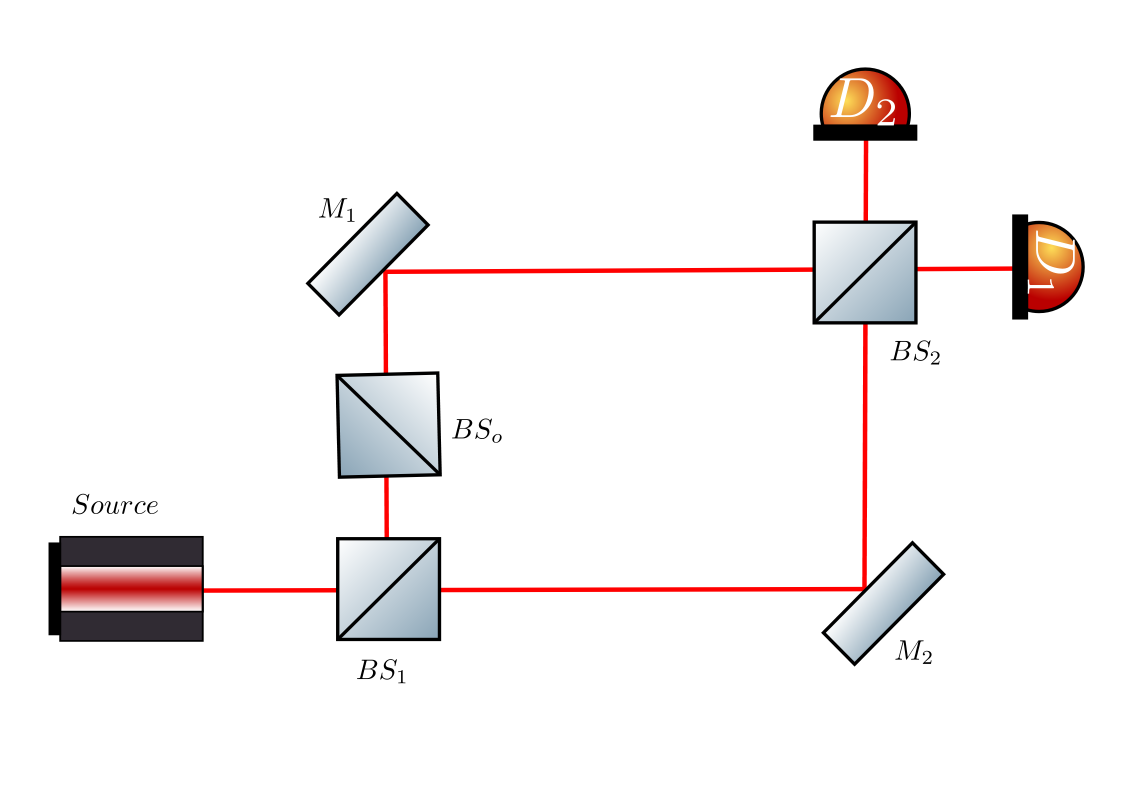
\includegraphics[width=\linewidth,height=7.5 cm]{images/machzenhderbs.png}
\caption{Mach-Zehnder interferometer with a $BS$ as imperfect transmitter.}
\label{bs vertical}
\end{figure}

Thus, let us assume that our imperfect transmitter is a beam splitter $BS_{o}$ whose transmission and reflection coefficients are $\cos(\theta_{o})$ and $i\sin(\theta_{o})$, respectively. When the photon in the state $\ket{2}$ interacts with our imperfect transmitter, its state is transformed as:

\begin{align}
\ket{2}\xrightarrow[\text{transmitter}]{\text{Imperfect}}i\sin(\theta_{o}) \ket{abs} +\cos(\theta_{o}) \ket{2}.
\end{align}

As the reflected photon goes out of the paths of the interferometer, and, thus out of reach of the remaining optical components, it might be considered as if it were absorbed by this component of the device. So, we denote its state by the vector $\ket{abs}$ as in the case of the states of truly absorbed photons of the previous experiments. With that in mind  now our model is an analogous form to those cases of the previous sections.

Assuming the photon enters the interferometer though the horizontal channel, i.e being in the initial state $\ket{1}$, The evolution of the state goes as follows:



\begin{align*}
&\ket{1}\xrightarrow{\text{BS1}}\cos(\theta_{1})\ket{1}+i\sin(\theta_{1})\ket{2}\\
&\xrightarrow{\text{BSo}}\cos(\theta_{1})\ket{1}+i\sin(\theta_{1})\left[\cos(\theta_{o})\ket{2}+i\sin(\theta_{o})\ket{abs}\right]\\ &\xrightarrow{\text{Mirrors}} \cos(\theta_{1})e^{i\gamma_{1}}\ket{2}+i\sin(\theta_{1})\cos(\theta_{o})e^{i\gamma_{2}}\ket{1}-\sin(\theta_{1})\sin(\theta_{o})\ket{abs}\\ &\xrightarrow{\text{BS2}}\cos(\theta_{1})e^{i\gamma_{1}}\left[\cos(\theta_{2})\ket{2}
+i\sin(\theta_{2})\ket{1}\right]+i\sin(\theta_{1})\cos(\theta_{o})e^{i\gamma_{2}}\\
&\times \left[\cos(\theta_{2})\ket{1}+i\sin(\theta_{2})\ket{2}\right]-\sin(\theta_{1})\sin(\theta_{o})\ket{abs}\\
&=(\cos(\theta_{1})e^{i\gamma_{1}}\cos(\theta_{2})-\sin(\theta_{1})\sin(\theta_{2})\cos(\theta_{o})e^{i\gamma_{2}})\ket{2}-\sin(\theta_{1})\sin(\theta_{o})\ket{abs}\\ &+(i\cos(\theta_{1})\sin(\theta_{2})e^{i\gamma_{1}}+
 i \sin(\theta_{1})\cos(\theta_{o})\cos(\theta_{2})e^{i\gamma_{2}})\ket{1}.\numberthis
\end{align*}
The detection probabilities can now be readily written:
\begin{align}
 P_{2D_{1}}&=|\cos(\theta_{1})\sin(\theta_{2})+ e^{i(\gamma_{2}-\gamma_{1})}\cos(\theta_{o}) \sin(\theta_{1})\cos(\theta_{2})|^2,\\
 P_{2D_{2}}&=|\cos(\theta_{1})\cos(\theta_{2})- e^{i(\gamma_{2}-\gamma_{1})}\cos(\theta_{o}) \sin(\theta_{1})\sin(\theta_{2})|^2,\\
 P_{2abs}&=|\sin(\theta_{o}) \sin(\theta_{1})|^2.
\end{align}

It is worthwhile noting that $P_{2D_{1}}$ and $P_{2D_{2}}$ do not depend on $\gamma_{1}$ and $\gamma_{2}$ independently but only on the difference $\gamma_{2}-\gamma_{1}$ meaning that the detection probabilties are only sensitive to the relative phases introduced by the mirrors. Adittionally, as it might be expected the absortion probability depends only on the parameters of $BS_{1}$ and $BS_{o}$.

We show the plots for the detection probabilities $P_{2abs}$, $P_{2D_{1}}$ and $P_{2D_{2}}$ in Fig. \ref{P_bs}, as functions of $\theta_{1}$ and $\theta_{2}$ for the particular values of $\theta_{o}=\frac{\pi}{3}$ and $\gamma_{2}-\gamma_{1}=\pi$. There we can see the oscilatory behavious in both parameters:



\begin{figure}[H]
\centering
\begin{subfigure}[b]{0.45\linewidth}
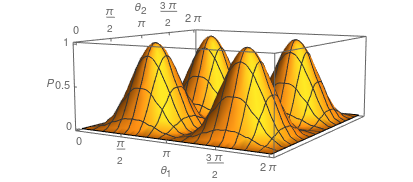
\includegraphics[width=\linewidth,height=2.8 cm]{images/P1abs.png}
\caption{$P_{2abs}$}
\label{fig:BS2}
\end{subfigure}
\begin{subfigure}[b]{0.45\linewidth}
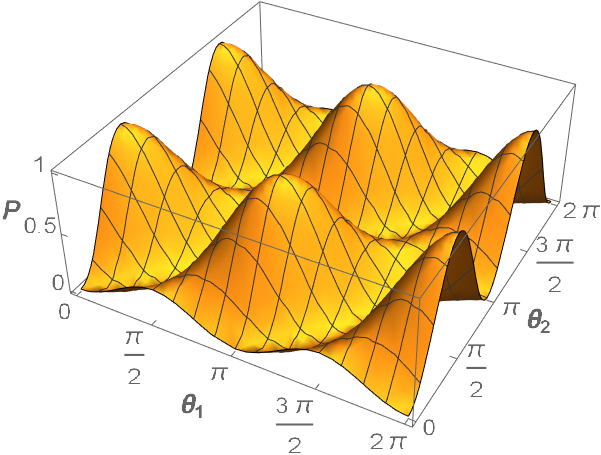
\includegraphics[width=\linewidth,height=2.8 cm]{images/P1d1.png}
\caption{$P_{2D_{1}}$}
\label{fig:westminster_aerea}
\end{subfigure}
\begin{subfigure}[b]{0.45\linewidth}
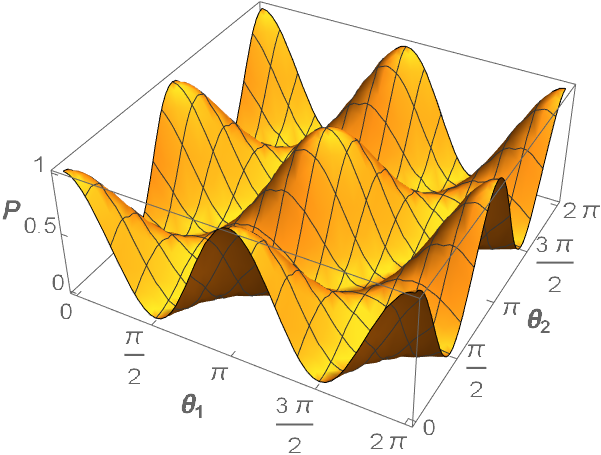
\includegraphics[width=\linewidth,height=2.8 cm]{images/P1d2.png}
\caption{$P_{2D_{2}}$}
\label{fig:BS2}
\end{subfigure}
\caption{Probability distributions of detection and absorption of the photon with the imperfect absorber placed in the vertical path. In these plots $\theta_{o}=\frac{\pi}{3}$ and $\gamma_{2}-\gamma_{1}=\pi$.}
\label{P_bs}
\end{figure}




Repeating the same calculation with the beam splitter $BS_{o}$ in the horizontal path we obtain the following detection probabilities



\begin{align}
P_{1D_{1}}&=|e^{i(\gamma_{1}-\gamma_{2})}\cos(\theta_{1})\sin(\theta_{2})\cos(\theta_{o})+ \sin(\theta_{1})\cos(\theta_{2})|^2, \\
P_{1D_{2}}&=|\cos(\theta_{1})\cos(\theta_{o})\cos(\theta_{2})e^{i(\gamma_{1}-\gamma_{2})}- \sin(\theta_{1})\sin(\theta_{2})|^2,\\
P_{1abs}&=|\sin(\theta_{o}) \cos(\theta_{1})|^2 .
\end{align}

which are shown graphically in Fig. \ref{P_bs2} as functions of $\theta_{1}$ and $\theta_{2}$, for the same values of $\theta_{o}$ and $\gamma_{2}-\gamma_{1}$ than those of Fig. \ref{P_bs}. We can see they are quite different, valleys in one are hills on the other and one the reasons is that we are always launching the incident photon from the same input channel, so that the initial conditions are not symetrical.

\begin{figure}[t]
\centering
\begin{subfigure}[b]{0.45\linewidth}
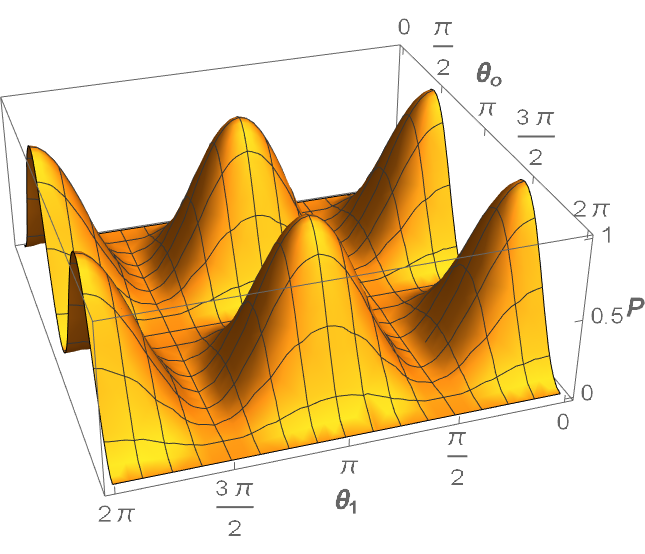
\includegraphics[width=\linewidth]{images/P11abs.png}
\caption{$P_{1abs}$}
\label{fig:BS1}
\end{subfigure}
\begin{subfigure}[b]{0.45\linewidth}
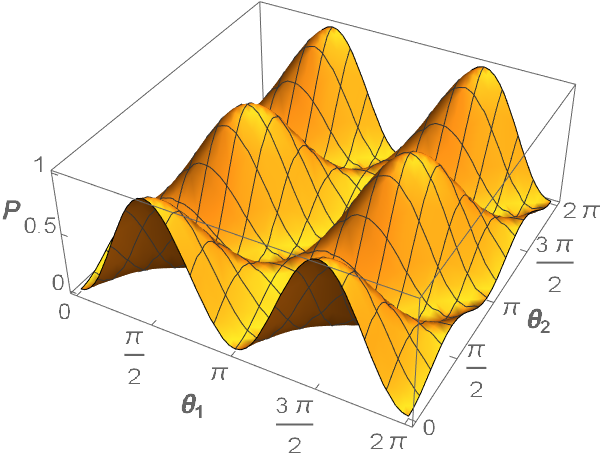
\includegraphics[width=\linewidth ,height=3 cm]{images/P11d1.png}
\caption{$P_{1D_{1}}$}
\label{fig:westminster_aerea}
\end{subfigure}
\begin{subfigure}[b]{0.45\linewidth}
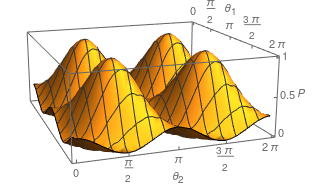
\includegraphics[width=\linewidth]{images/P11d2.png}
\caption{$P_{1D_{2}}$}
\label{fig:BS1}
\end{subfigure}
\caption{Probability distributions of detection and absorption of the photon with the imperfect absorber placed in the horizontal path. In these plots $\theta_{o}=\frac{\pi}{3}$ and $\gamma_{2}-\gamma_{1}=\pi$.}
\label{P_bs2}
\end{figure}



Our results are totally consistent with those reported in \cite{zuri,azuri} by taking $\beta=\cos(\theta_{o})$, $\alpha=i \sin(\theta_{o})$ and $\gamma_{2}-\gamma_{1}=0$. One of the advantages of this setup is that the ``absorbed'' photon, is not really absorbed but redirected through another path and can be monitored as well, by a third detector, say $D_{abs}$, enabling, thus the posibility of correlating the absorption and detection probabilities.

\section{Replacing the bomb with $N$ beam splitters }


\begin{figure}[H]
\centering
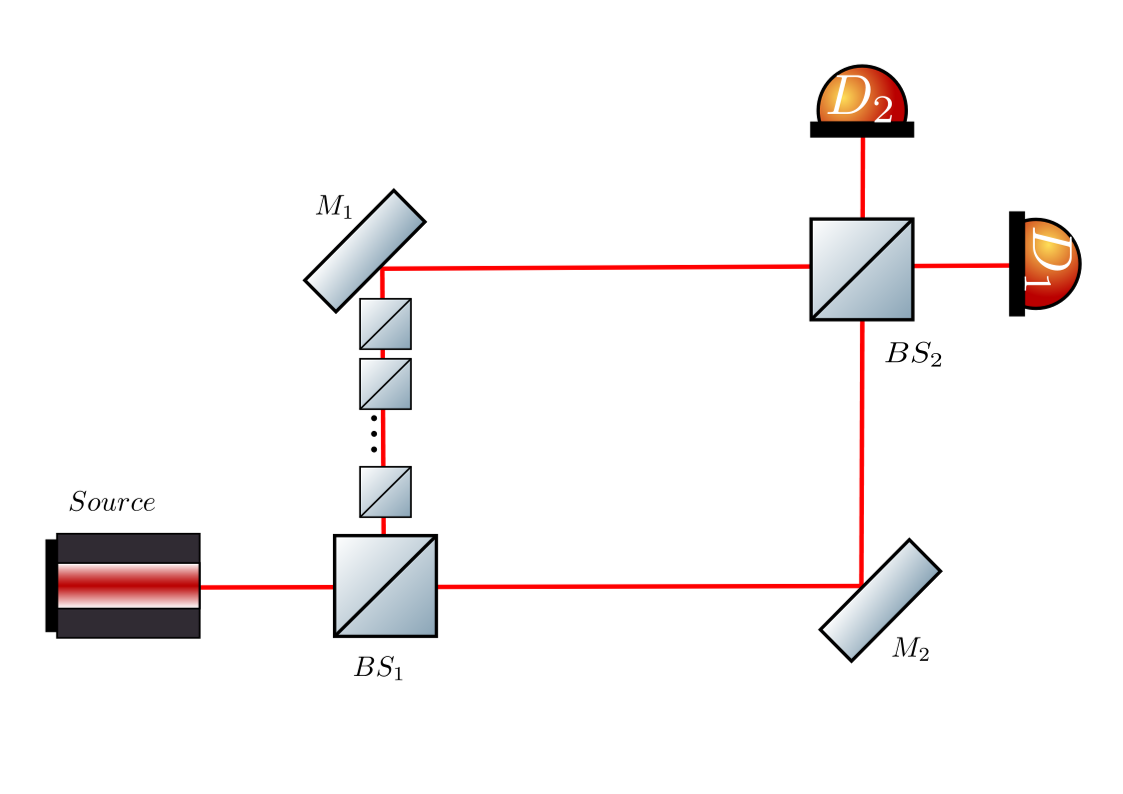
\includegraphics[width=\linewidth,height=8 cm]{images/machzenhderBSS.png}
\caption{Mach-Zehnder with $N$ $BS$ as imperfect transmitter.}
\label{N_bs}
\end{figure}


In this section, we analyze the case in which an array of $N$ beam splitters are place along one path of the interferometer (see figure \ref{N_bs}). Let us denote the beam splitters in this array by $BS_{i}$, where $i=1,2,3,4,5,...,N+2$. Assuming that the reflected photon in either beam splitter $BS_{i}$ is ``absorbed'', we have that, the state of the photon initially in the state $\ket{2}$ is transformed into

\begin{align}
BS_{3}\ket{2}=\cos(\theta_{3})\ket{2}+i\sin(\theta_{3})\ket{abs}.
\end{align}

The next beam splitter only acts on the transmitted photon state, since, as explained in the previous section, if the photon is reflected then it goes out of the interferometer and does not interact with the optical elements any longer:
\begin{align}
BS_{4}(\cos(\theta_{3})\ket{2}+i\sin(\theta_{3})\ket{abs})&=\cos(\theta_{3})BS_{4}\ket{2}+i\sin(\theta_{3})\ket{abs},\\
BS_{4}BS_{3}\ket{2}&=\cos(\theta_{3})\cos(\theta_{4})\ket{2}+i A_{2}\ket{abs}.
\end{align}
where $A_{2}$ is the composed absorption coefficient for a two beam splitter array. The action of the rest of the beam splitters are equivalent
\begin{equation}
BS_{5}BS_{4}BS_{3}\ket{2}=\cos(\theta_{3})\cos(\theta_{4})\cos(\theta_{5})\ket{2}+iA_{3}\ket{abs},
\end{equation}

where $A_{3}$ is the absorption coefficient of the 3-BS array. Finally, for the  $N$ $BS$ array we have:

\begin{align*}
BS^{N}\ket{2}=BS_{N}...BS_{3}\ket{2}=\cos(\theta_{3})\cos(\theta_{4})\cos(\theta_{5})....\cos(\theta_{N})\ket{2} +i A_{N}\ket{abs}. \numberthis
\end{align*}

We can obtain $A_{N}$ by considering that everything that if the photon is not transmitted then it will be ``absorbed":

\begin{align}
BS^{N}\ket{2}&=\prod_{i=3}^{N+2} \cos(\theta_{i})\ket{2}+i A_{N} \ket{abs},\\
A_{N}&=\sqrt{1-\prod_{i=3}^{N+2}\cos^2(\theta_{i})}.
\end{align}

Following a similar procedure we could obtain a similar result if the $N$ $BS$ array is in the other arm of the interferometer,namely

\begin{align}
BS^{N}\ket{1}&=\prod_{i=3}^{N+2} \cos(\theta_{i})\ket{1}+i \sqrt{1-\prod_{i=3}^{N+2}\cos^2(\theta_{i})} \ket{abs}
\end{align}
 We now use this $N$ $BS$ array to model the imperfect absorber, we can calculate the evolution of a photon initially in state $\ket{1}$ through the interferometer, passing the set of $N$ beam splitters that replaced the bomb (placed in the vertical arm just after $BS_1$), being reflected by $M_1$ and $M_2$, recombined in $BS_2$ and finally going directly to detectors $D_1$ and $D_2$ as: 


\begin{align*}
&\ket{1}\xrightarrow{\text{BS1}}\cos(\theta_{1})\ket{1}+i\sin(\theta_{1})\ket{2}\\ &\xrightarrow{{BS^{N}}}\cos(\theta_{1})\ket{1}+i\sin(\theta_{1})\prod_{i=3}^{N+2} \cos(\theta_{i})\ket{2}-\sin(\theta_{1})\sqrt{1-\prod_{i=3}^{N+2}\cos^2(\theta_{i})}\ket{abs} \\ & \xrightarrow{{Mirrors}}\cos(\theta_{1})  e^{i \gamma_{1}}\ket{2}+i\sin(\theta_{1})\prod_{i=3}^{N+2} \cos(\theta_{i}) e^{i \gamma_{2}}\ket{1}\\
&-\sin(\theta_{1})\sqrt{1-\prod_{i=3}^{N+2}\cos^2(\theta_{i})}\ket{abs} \\ & \xrightarrow{{BS2}}(\cos(\theta_{1})\cos(\theta_{2})e^{i \gamma_{1}}-\sin(\theta_{1})\sin(\theta_{2})e^{i \gamma_{2}}\prod_{i=3}^{N+2} \cos(\theta_{i}))\ket{2}\\ &+ i(\cos(\theta_{1})\sin(\theta_{2})e^{i \gamma_{1}}+\cos(\theta_{2})\sin(\theta_{1})e^{i \gamma_{2}}\prod_{i=3}^{N+2} \cos(\theta_{i}))\ket{1}\\ &-\sin(\theta_{1})\sqrt{1-\prod_{i=3}^{N+2}\cos^2(\theta_{i})}\ket{abs}.
\end{align*}
 
The probabilities of detection at each of the detectors and the probability of absorption are given by:

\begin{align}
P_{2D_{1}}&=|\cos(\theta_{1})\sin(\theta_{2})+\cos(\theta_{2})\sin(\theta_{1})e^{i (\gamma_{2}-\gamma_{1})}\prod_{i=3}^{N+2} \cos(\theta_{i})|^2,\\
P_{2D_{2}}&=|\cos(\theta_{1})\cos(\theta_{2})-\sin(\theta_{1})\sin(\theta_{2})e^{i (\gamma_{2}-\gamma_{1})}\prod_{i=3}^{N+2} \cos(\theta_{i})|^2,\\
P_{2abs}&=\sin^2(\theta_{1})\left(1-\prod_{i=3}^{N+2}\cos^2(\theta_{i})\right).
\end{align}


To know wheter the or  not the array of beam splitters is there or not, is no different from the previous sections as this case would simply correspond to $\beta=\prod_{i=3}^{N+2} \cos(\theta_{i})$.

\afterpage{\blankpage}
\chapter{A time-dependent transmitter}

In this chapter we will substitute the bomb in the Elitzur-Vaidman experiment with an object whose transmission and absorption coefficients depend on time, this object will be an optical chopper whose time dependence is discrete. Let us begin by analyzing the optical chopper as a perfect absorber.

\section{Replacing the bomb with an optical chopper }
 

An optical chopper is a device that periodically interrupts light. It is usually a disk with holes rotating with a certain frequency (which can vary in time). We can model the presence of a chopper interrupting the pass of light with and object whose coefficient of transmission  varies as a square wave  $f(t)=\frac{sgn(\sin(wt))+1}{2}$, where $\omega$ is the angular frequency of the optical chopper multiplied by the number of ``hole-material" pairs that we assume are the same size.

 \begin{figure}[h!]
\centering
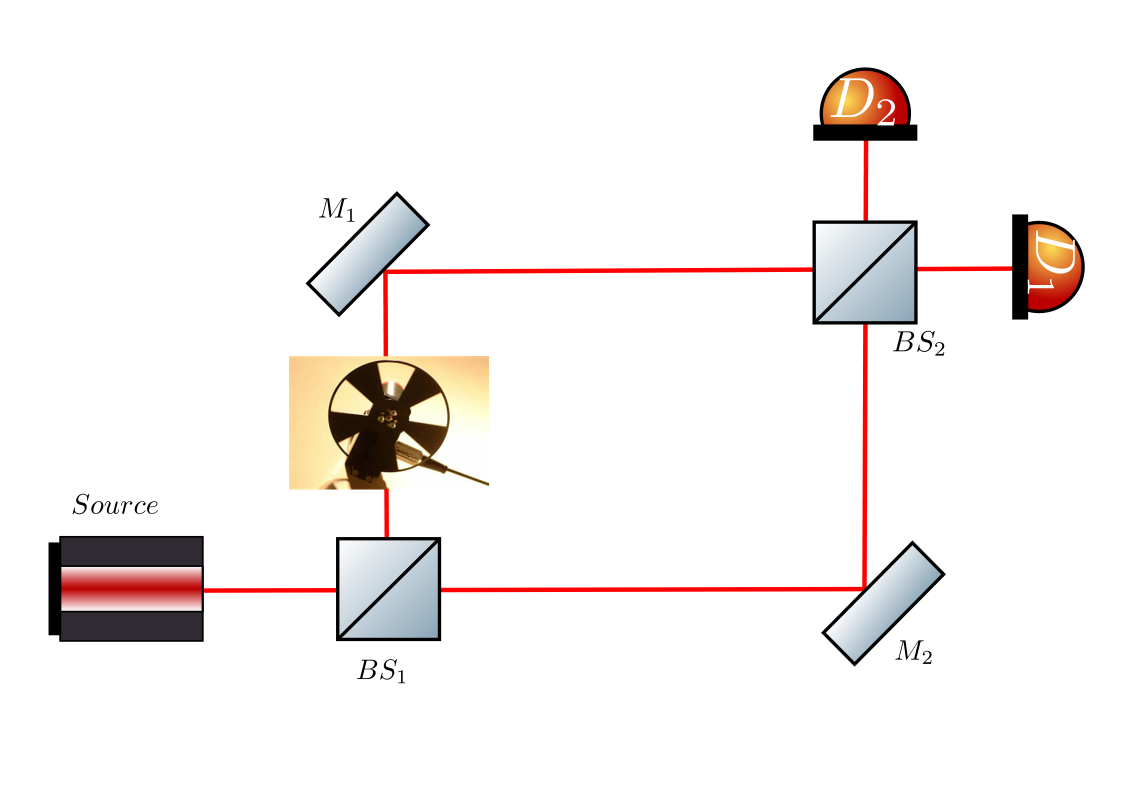
\includegraphics[width=\linewidth]{images/machzenhderchopper.png}
\caption{Mach-Zehnder interferometer with an optical chopper as an imperfect absorber.}
\label{chopper}
\end{figure}

We will be ignoring diffraction effects, a consequence of modeling it like this is that consecutive optical choppers become the product of square waves, and products of square waves is again a square wave, so modeling many choppers would be the same as modeling one with that effective frequency and duty-cycle. In this section, we intend to analyze the Mach-Zehnder interferometer with a chopper replacing the bomb in the Elitzur and Vaidmand experiment, as in Fig. \ref{chopper}, the chopper introduces a discrete-time dependence, therefore we will be alternating between two different probability distributions.


We can model our optical chopper by using an operator $C_{i}$ where $i$ is the path where the chopper is placed, such that in our base(where $i=1,2$ and $i \neq j$):

\begin{equation}
C_{i}\ket{i}=f(t)\ket{i},\qquad C_{j}\ket{i}=\ket{i}.
\end{equation}

Since we are modeling the hole as a transparent object, the operator $C_i$ is unitary in the 'hole' cycle.  This is indeed fullfilled as the square of the sign function is always one.


From there we can see that it is a unitary matrix whenever the sine is in the positive cycle, and it becomes null in the negative cycle, that happens because in the negative cycle we have total absorption. The absorption coefficient would  be:  

\begin{align}
 \alpha=1-f,\qquad \alpha=\frac{1-sgn(\sin(wt))}{2},
\end{align}

We will now analyze a Mach-Zehnder interferometer using a chopper as a time-dependent absorber. The chopper will be placed on the vertical path, and our photon will go into the interferometer using the horizontal path



\begin{align*}
&\ket{1}\xrightarrow{\text{BS1}}\cos(\theta_{1})\ket{1}+i\sin(\theta_{1})\ket{2}\\ &\xrightarrow{\text{Chopper}}\cos(\theta_{1})\ket{1}+i\sin(\theta_{1})f\ket{2}+i\sin(\theta_{1})\alpha\ket{abs}\\ &\xrightarrow{\text{Mirrors}} \cos(\theta_{1})e^{i\gamma_{1}}\ket{2}+i\sin(\theta_{1})f e^{i\gamma_{2}}\ket{1}+i\sin(\theta_{1})\alpha\ket{abs}\\& \xrightarrow{\text{BS2}}\cos(\theta_{1})e^{i\gamma_{1}}(\cos(\theta_{2})\ket{2}\\
&+i\sin(\theta_{2})\ket{1})+i\sin(\theta_{1})e^{i\gamma_{2}}f(\cos(\theta_{2})\ket{1}+i\sin(\theta_{2})\ket{2})+i\sin(\theta_{1})\alpha\ket{abs}\\
& = i(e^{i\gamma_{1}}\cos(\theta_{1})\sin(\theta_{2})+f e^{i\gamma_{2}}\sin(\theta_{1})\cos(\theta_{2}))\ket{1}+(\cos(\theta_{1})\cos(\theta_{2}) e^{i\gamma_{1}} \\&  -\sin(\theta_{1})\sin(\theta_{2})f e^{i \gamma_{2}})\ket{2}+i\sin(\theta_{1})\alpha\ket{abs}. \numberthis
\end{align*}



A plot for the detection probabilities is shown in Fig. \ref{Pchopper}. As we mentioned before, the system is alternating between two probability distributions. We can see those for each of the possible states in the figure. It is worth noting that the absorption graph alternates between the one shown and no absorption:



\begin{figure}[t!]
\centering
\begin{subfigure}[b]{0.45\linewidth}
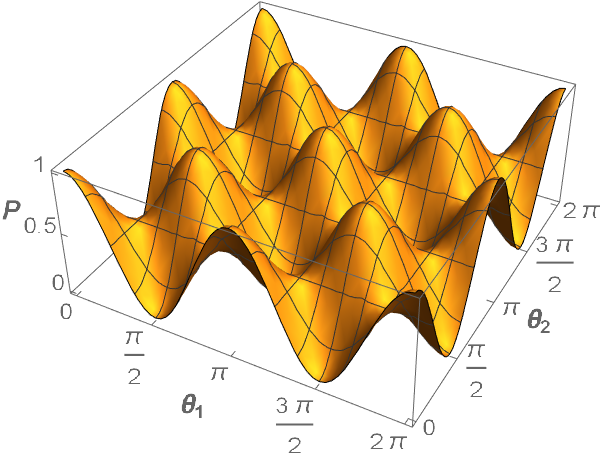
\includegraphics[width=\linewidth,height=3 cm]{images/Pc2D22.png}
\caption{$P_{2D_{2}}$ in the second cycle}
\label{fig:BS1}
\end{subfigure}
\begin{subfigure}[b]{0.45\linewidth}
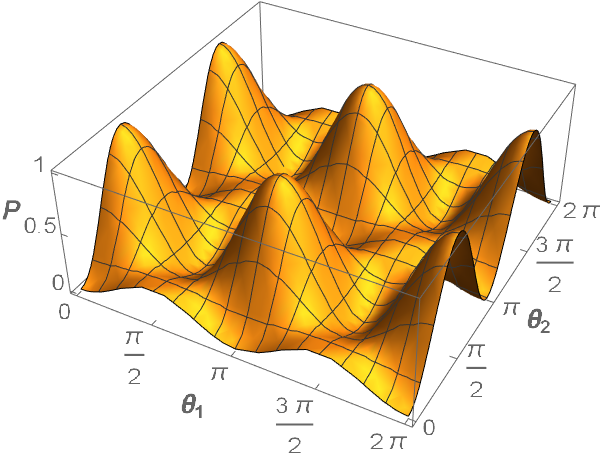
\includegraphics[width=\linewidth,height=3 cm]{images/Pc2D11.png}
\caption{$P_{2D_{1}} $ in the first cycle}
\label{fig:westminster_aerea}
\end{subfigure}
\begin{subfigure}[b]{0.45\linewidth}
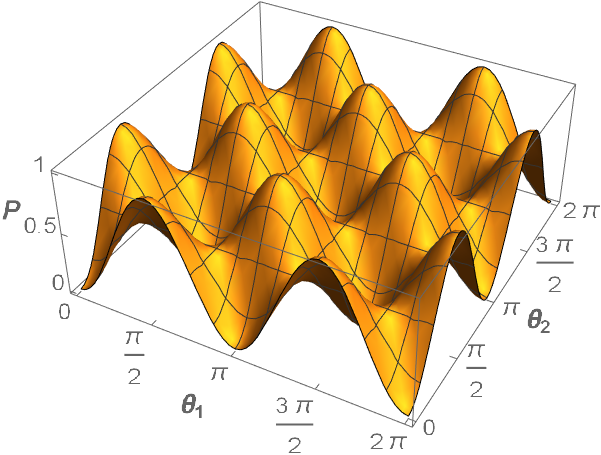
\includegraphics[width=\linewidth,height=3 cm]{images/Pc2D12.png}
\caption{$P_{2D_{1}} $ in the second cycle }
\label{fig:BS1}
\end{subfigure}
\begin{subfigure}[b]{0.45\linewidth}
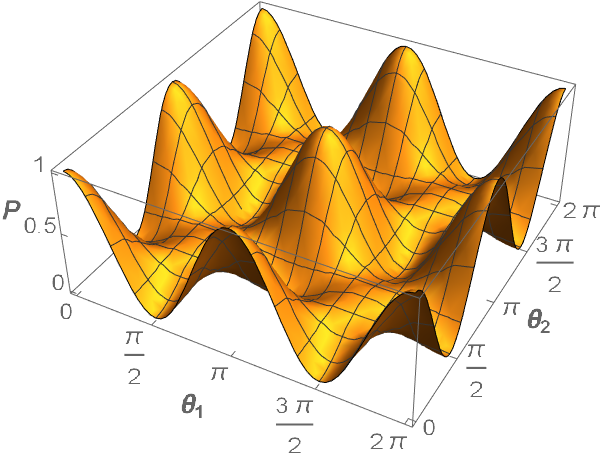
\includegraphics[width=\linewidth,,height=3 cm]{images/Pc2D21.png}
\caption{$P_{2D_{2}}$ in the first cycle }
\label{fig:BS1}
\end{subfigure}
\begin{subfigure}[b]{0.45\linewidth}
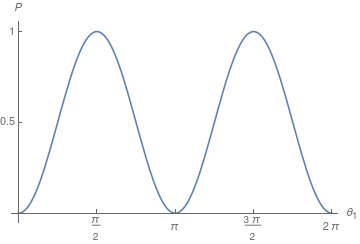
\includegraphics[width=\linewidth,height=3 cm]{images/Pc2Abs.png}
\caption{$P_{2abs}$}
\label{fig:BS1}
\end{subfigure}

\caption{Probability distributions of detection and absorption of the photon at detectors $D_{1}$ and $D_{2}$ with an optical chopper whose solid material is totally absorbent  placed in the vertical path. In these plots  $\gamma_{2}-\gamma_{1}=\frac{\pi}{2}$.}
\label{Pchopper}
\end{figure}


\begin{align}
&P_{2D_{1}}=|e^{i\gamma_{1}}\cos(\theta_{1})\sin(\theta_{2})+f e^{i\gamma_{2}}\sin(\theta_{1})\cos(\theta_{2})|^2,\\
&P_{2D_{2}}=|\cos(\theta_{1})\cos(\theta_{2})e^{i\gamma_{1}}- f \sin(\theta_{1})\sin(\theta_{2})e^{i\gamma_{2}}|^2,\\
&P_{2abs}=|\alpha \sin(\theta_{1})|^2.
\end{align}

Which can be rewritten as:
\begin{align*}
& P_{2D_{1}}=\cos^2(\theta_{1})\sin^2(\theta_{2})+f^2 \sin^2(\theta_{1})\cos^2(\theta_{2})+\\
&\frac{f \sin(2\theta_{1})\sin(2\theta_{2})\cos(\gamma_{1}-\gamma_{2})}{2}, \numberthis{}\\
& P_{2D_{2}}=\cos^2(\theta_{1})\cos^2(\theta_{2})+ f^2 \sin^2(\theta_{1})\sin^2(\theta_{2})-\\
&\frac{f \sin(2\theta_{1})\sin(2\theta_{2})\cos(\gamma_{1}-\gamma_{2})}{2},\numberthis{} \\
& P_{2abs}=\alpha^2 \sin^2(\theta_{1}).\numberthis{}
\end{align*}

By the same procedure having the chopper in the horizontal path, one can obtain the following results which are shown in Fig. \ref{P2chopper}, for each of the possible states of the system
 
\begin{figure}[h!]
\centering

\begin{subfigure}[b]{0.35\linewidth}
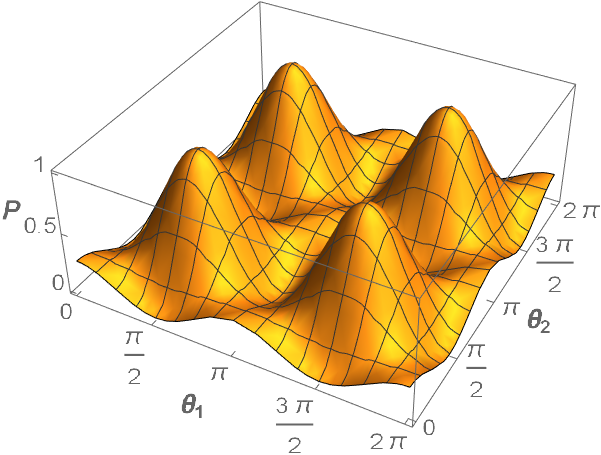
\includegraphics[width=\linewidth,height=3 cm]{images/Pc1D21.png}
\caption{$P_{1D_{2}}$ in the first cycle }
\label{fig:BS1}
\end{subfigure}
\begin{subfigure}[b]{0.35\linewidth}
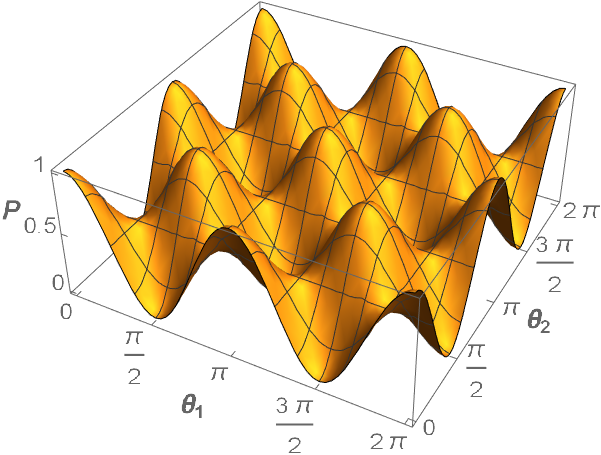
\includegraphics[width=\linewidth,height=3 cm]{images/Pc1D22.png}
\caption{$P_{1D_{2}}$ in the second cycle}
\label{fig:BS1}
\end{subfigure}
\begin{subfigure}[b]{0.35\linewidth}
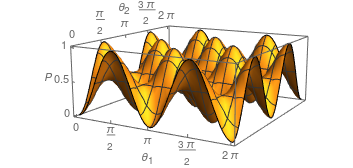
\includegraphics[width=\linewidth,height=3 cm]{images/Pc1D11.png}
\caption{$P_{1D_{1}} $ in the first cycle}
\label{fig:westminster_aerea}
\end{subfigure}
\begin{subfigure}[b]{0.35\linewidth}
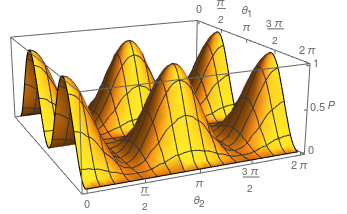
\includegraphics[width=\linewidth,height=3 cm]{images/Pc1D12.png}
\caption{$P_{1D_{1}} $in the second cycle }
\label{fig:BS1}
\end{subfigure}
\begin{subfigure}[b]{0.35\linewidth}
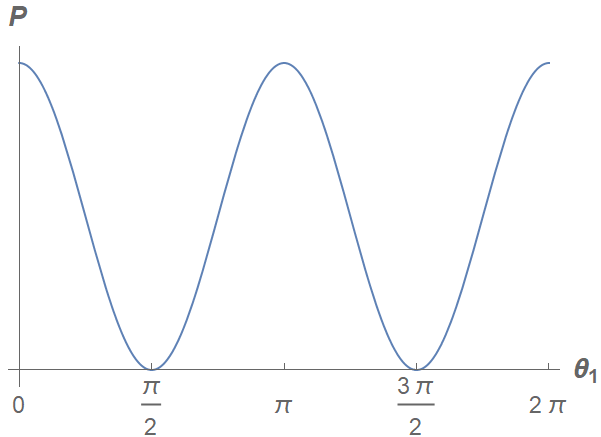
\includegraphics[width=\linewidth,height=3 cm]{images/Pc1Abs.png}
\caption{$P_{1abs}$}
\label{fig:BS1}
\end{subfigure}
\caption{Probability distributions of detection and absorption of the photon at detectors $D_{1}$ and $D_{2}$ with an optical chopper whose solid material is totally absorbent  placed in the horizontal path. In these plots  $\gamma_{2}-\gamma_{1}=\frac{\pi}{2}$.}
\label{P2chopper}
\end{figure}

\begin{align*}
& P_{1D_{1}}=\cos^2(\theta_{1})\sin^2(\theta_{2})f^2+ \sin^2(\theta_{1})\cos^2(\theta_{2})+\\
&\frac{f \sin(2\theta_{1})\sin(2\theta_{2})\cos(\gamma_{1}-\gamma_{2})}{2},\numberthis{}\\
& P_{1D_{2}}=\cos^2(\theta_{1})\cos^2(\theta_{2})f^2+ \sin^2(\theta_{1})\sin^2(\theta_{2})-\\
&\frac{f \sin(2\theta_{1})\sin(2\theta_{2})\cos(\gamma_{1}-\gamma_{2})}{2},\numberthis{}\\
& P_{1abs}=\alpha^2 \cos^2(\theta_{1}). \numberthis{}
\end{align*}

Since $f^2=f$, we can write the difference of probabilities as:

\begin{align}
P_{1D_{1}}-P_{1D_{2}}=\alpha\left(\frac{\cos(2 \theta_{1})-\cos(2 \theta_{2})}{2}\right),\
P_{1D_{2}}-P_{2D_{2}}=\alpha\left(\frac{\cos(2 \theta_{1})+\cos(2 \theta_{2})}{2}\right).
\end{align}
 From there we can obtain either $\theta_{1}$  or $\theta_{2}$ :

 \begin{align}
&(P_{1D_{1}}-P_{1D_{2}})+(P_{1D_{2}}-P_{2D_{2}})=\alpha(\cos(2 \theta_{1})),\\
&(P_{1D_{1}}-P_{1D_{2}})-(P_{2D_{1}}-P_{2D_{2}})=-\alpha(\cos(2 \theta_{2})),\\
 &\theta_{1}=\frac{1}{2}\cos^{-1}\left[\frac{(P_{1D_{1}}-P_{2D_{1}})+(P_{1D_{2}}-P_{2D_{2}})}{\alpha}\right],\\
 &\theta_{2}=\frac{1}{2}\cos^{-1}\left[\frac{(P_{1D_{1}}-P_{2D_{1}})-(P_{1D_{2}}-P_{2D_{2}})}{\alpha}\right].
 \end{align}


\section{Optical chopper as imperfect absorber}

Previously we considered the ``material" part of the chopper as a perfect absorber. In this section,  we will generalize the results of the previos section. Instead of considering the material of the chopper with a transmission coeficient $\beta = 0$, we will take $\beta \neq 0$, i.e. it is a semitransparent material. Let us define: 
 

\begin{align}
f_{hole}&=\frac{1+sgn(\sin(wt))}{2},\\
f_{material}&=\left(\frac{1-sgn(\sin(wt))}{2} \right)\beta,\\
f&=f_{material}+f_{hole},
\end{align}


where $\beta$ is the transmission coefficient of the material part of our chopper. The operator used to describe our chopper is the same as in the previous section, we define:

\vspace{0.5cm}
\begin{equation}
a=\left(\frac{1-sgn(\sin(wt))}{2}\right) \alpha,
\end{equation}
\vspace{0.5cm}

where $\alpha$ is the absorption coefficient of the material part of our chopper, by using this notation we have the same case as in the previous section, except this time $f^2 \neq 1$ :

\begin{align}
|a|^2&=a \alpha.\\
|f_{material}|^2&=f_{material} \beta,
\end{align}

which we can generalize to obtain:

\begin{align}
|a|^n&=a\alpha^{n-1},\\
|f_{material}|^n&=f_{material} \beta^{n-1},
\end{align}
so we have:

\begin{equation}
|f|^2=  \frac{\abs{\alpha}^2}{2} sgn(\sin(wt)) +\frac{1+\abs{\beta}^2}{2}.
\end{equation}



Substituting in the previous section yields the probability distributions shown in Fig. \ref{P3chopper}:

\begin{figure}[h]
\centering

\begin{subfigure}[b]{0.40\linewidth}
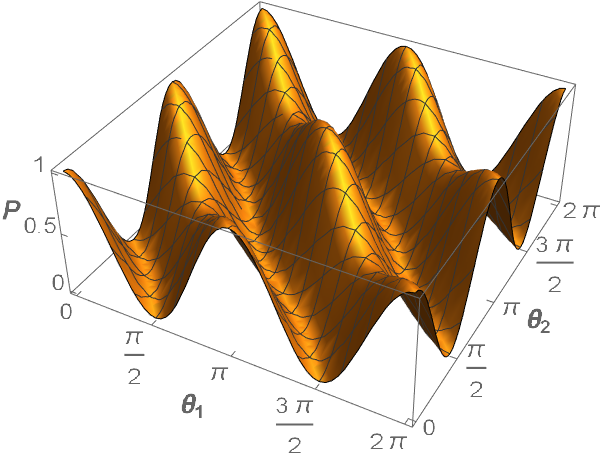
\includegraphics[width=\linewidth,height=3 cm]{images/pcd21.png}
\caption{$P_{1D_{2}}$ in the first cycle }
\label{fig:BS1}
\end{subfigure}
\begin{subfigure}[b]{0.40\linewidth}
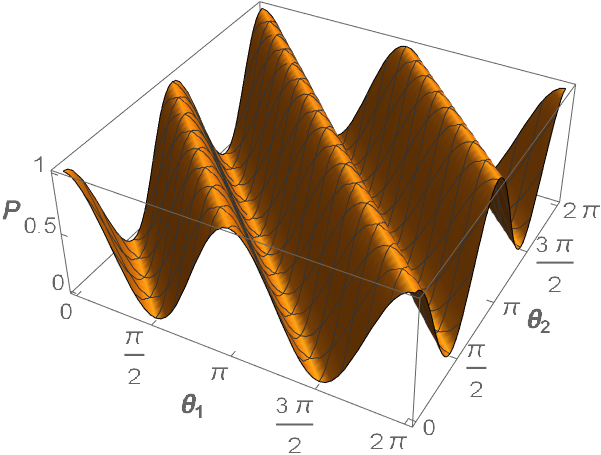
\includegraphics[width=\linewidth,height=3 cm]{images/pcd22.png}
\caption{$P_{1D_{2}}$ in the second cycle}
\label{fig:BS1}
\end{subfigure}
\begin{subfigure}[b]{0.40\linewidth}
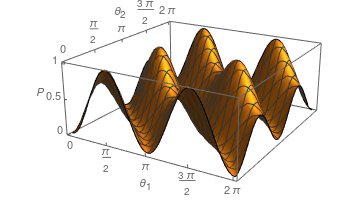
\includegraphics[width=\linewidth,height=3 cm]{images/pcd11.png}
\caption{$P_{1D_{1}} $ in the first cycle}
\label{fig:westminster_aerea}
\end{subfigure}
\begin{subfigure}[b]{0.40\linewidth}
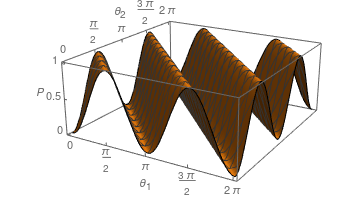
\includegraphics[width=\linewidth,height=3 cm]{images/pcd12.png}
\caption{$P_{1D_{1}} $ in the second cycle }
\label{fig:BS1}
\end{subfigure}
\begin{subfigure}[b]{0.40\linewidth}
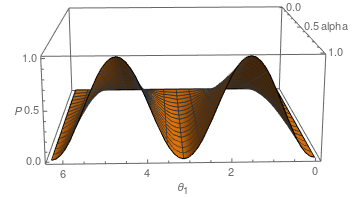
\includegraphics[width=\linewidth,height=3 cm]{images/pcabs.png}
\caption{$P_{1abs}$}
\label{fig:BS1}
\end{subfigure}
\caption{Probability distributions of detection and absorption of the photon with an optical chopper whose solid material is totally absorbent  placed in the horizontal path. In these plots  $\gamma_{2}-\gamma_{1}=0 $ and $\beta=0.5$.}
\label{P3chopper}
\end{figure}


\begin{align*}
&P_{1D_{1}}=\cos^2(\theta_{1})\sin^2(\theta_{2})\abs{f}^2+ \sin^2(\theta_{1})\cos^2(\theta_{2})\\
&+\frac{\Re{f} \sin(2\theta_{1})\sin(2\theta_{2})\cos(\gamma_{1}-\gamma_{2})}{2},\numberthis{}\\
&P_{1D_{2}}=\cos^2(\theta_{1})\cos^2(\theta_{2})\abs{f}^2+ \sin^2(\theta_{1})\sin^2(\theta_{2})\\
&-\frac{\Re{f} \sin(2\theta_{1})\sin(2\theta_{2})\cos(\gamma_{1}-\gamma_{2})}{2},\numberthis{}\\
&P_{1abs}=\abs{\alpha}^2 \cos^2(\theta_{1}).\numberthis{}
\end{align*}


When the optical chopper is in the vertical path we obtain the following detection probabilities. The probability distributions are shown in Fig. \ref{P4chopper}:

\begin{figure}[!h]
\centering

\begin{subfigure}[b]{0.40\linewidth}
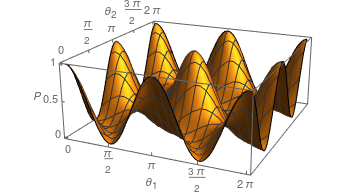
\includegraphics[width=\linewidth,height=3 cm]{images/p1cd21.png}
\caption{$P_{2D_{2}}$ in the first cycle }
\label{fig:BS1}
\end{subfigure}
\begin{subfigure}[b]{0.40\linewidth}
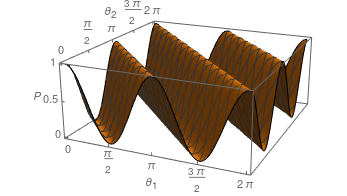
\includegraphics[width=\linewidth,height=3 cm]{images/p1cd22.png}
\caption{$P_{2D_{2}}$ in the second cycle}
\label{fig:BS1}
\end{subfigure}
\begin{subfigure}[b]{0.40\linewidth}
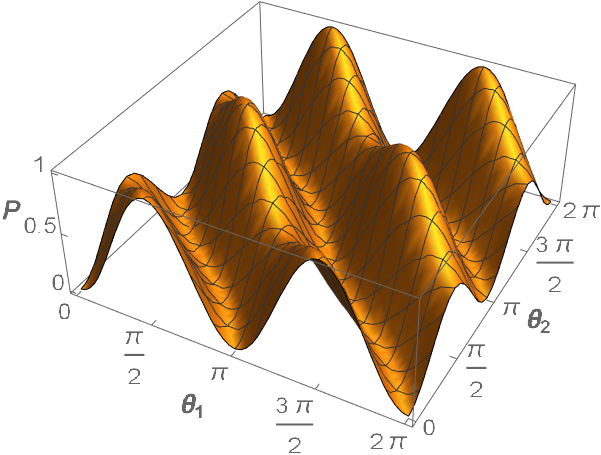
\includegraphics[width=\linewidth,height=3 cm]{images/p1cd11.png}
\caption{$P_{2D_{1}} $ in the first cycle}
\label{fig:westminster_aerea}
\end{subfigure}
\begin{subfigure}[b]{0.40\linewidth}
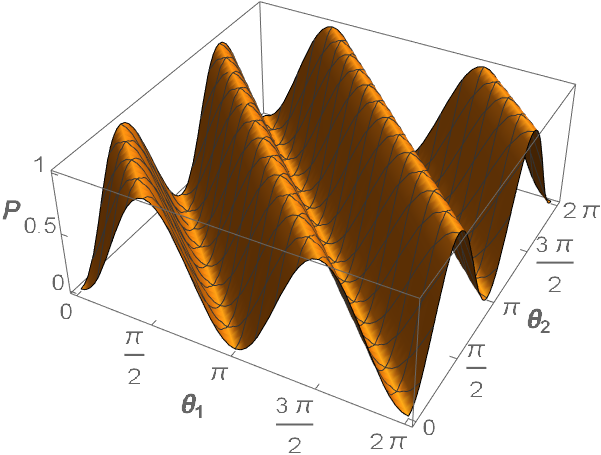
\includegraphics[width=\linewidth,height=3 cm]{images/p1cd12.png}
\caption{$P_{2D_{1}} $ in the second cycle }
\label{fig:BS1}
\end{subfigure}
\begin{subfigure}[b]{0.40\linewidth}
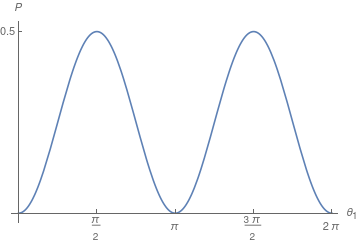
\includegraphics[width=\linewidth,height=3 cm]{images/p1cabs.png}
\caption{$P_{2abs}$}
\label{fig:BS1}
\end{subfigure}
\caption{Probability distributions of detection and absorption of the photon with an optical chopper whose solid material is totally absorbent  placed in the vertical path. In these plots  $\gamma_{2}-\gamma_{1}=0 $ and $\beta=0.5$.}
\label{P4chopper}
\end{figure}

\begin{align*}
&P_{2D_{1}}=\cos^2(\theta_{1})\sin^2(\theta_{2})+\abs{f}^2 \sin^2(\theta_{1})\cos^2(\theta_{2})\\
&+\frac{\Re{f} \sin(2\theta_{1})\sin(2\theta_{2})\cos(\gamma_{1}-\gamma_{2})}{2},\numberthis{}\\
&P_{2D_{2}}=\cos^2(\theta_{1})\cos^2(\theta_{2})+ \abs{f}^2 \sin^2(\theta_{1})\sin^2(\theta_{2})\\
&-\frac{\Re{f} \sin(2\theta_{1})\sin(2\theta_{2})\cos(\gamma_{1}-\gamma_{2})}{2},\numberthis{}\\
&P_{2abs}=\abs{\alpha}^2 \sin^2(\theta_{1}).\numberthis{}
\end{align*}

As explored in this section an optical chopper can be modeled as a square wave, basically, as the evolution of the system in this model is discrete and periodic the probability distribution of the system will be oscillating between the probability distribution of a semitransparent object and that of a transparent object.

\chapter[High-efficiency Mach-Zehnder Interferometer]{High-efficiency  Mach-Zehnder interferometer  }
 
 The notation previously used is not popular when dealing with nested interferometers. To be consistent with the existing literature we will use the same notation as Kwait et al. \cite{5}, where the arrangement shown in Fig. \ref{Nmach}, we see from the figure that we will have $N$ beam splitters and $N-1$ absorbers before the output:
 
 
Instead of using the Horizontal-Vertical basis, we will use a path A -path B basis. That is an ``up-down" basis, we will use $\ket{1}$ for path $a$ and $\ket{2}$ for path $b$. The main advantage of using this basis is that the mirror matrices are proportional to the identity because they keep our photon on the same path.
 
 
 In order to use the same beam splitter matrix as before and be consistent with the literature \cite{5}, we choose the reflectivity of the $N$ $BS$ to be modeled by $cos(\theta)$ instead of $i\sin(\theta)$, as a consequence the transmissivity is now $i\sin(\theta)$.  We will model our imperfect absorber using a non-unitary diagonal matrix just as was done by  Azuma \cite{Azuma}. Azuma used a matrix of the form, where $n=\abs{\beta}^{2}$, where $\beta$ is the transmissivity:
 
 \begin{equation}
 A_{Azuma}=\begin{pmatrix} \sqrt{n} & 0\\0& 1\end{pmatrix}.
\label{absorber}
 \end{equation}

Since we are using a $BS$ as an imperfect absorber a more suitable option would be :
\begin{equation}
 A_{BS}=\begin{pmatrix} \sin(\theta) & 0\\0& 1\end{pmatrix}.
\label{absorber1}
\end{equation}

\begin{figure}[H]
\centering
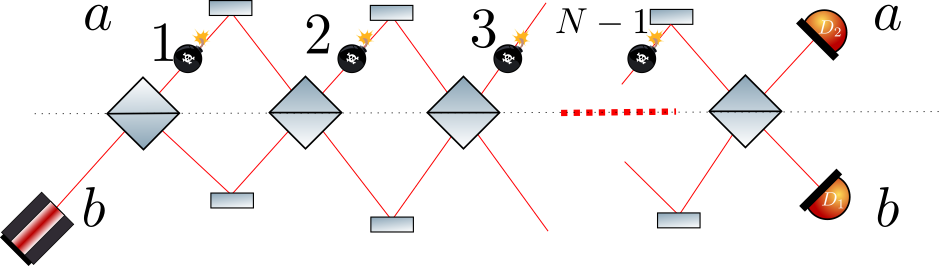
\includegraphics[width=\linewidth]{images/nmach2.png}
\caption{Nested Mach-Zehnder interferometer  with identical imperfect absorbers.}
\label{Nmach}
\end{figure}
The final state can be obtained by applying the operators corresponding to each of the optical elements involved to the initial state $\ket{2}$. We consider both mirrors to be identical so that the phase they induce ends up being a global phase which does not affect the probabilities. First, we study the case with no obstacles in any of the arms of the interferometer. The evolution of the initial state $\ket{2}$ can be calculated by applying on it the matrix of each $BS$, but notice that the multiplication of two $BS$ matrices is

\begin{align*}
BS_{i} \times BS_{i+1}&=\begin{pmatrix} \cos(\theta_{i}) & i \sin(\theta_{i}) \\ i \sin(\theta_{i}) & \cos(\theta_{i}) \end{pmatrix}  
\begin{pmatrix} \cos(\theta_{i+1}) & i \sin(\theta_{i+1}) \\ i \sin(\theta_{i+1}) & \cos(\theta_{i+1}) \end{pmatrix},\\
&=\begin{pmatrix} \cos(\theta_{i}+\theta_{i+1}) & i \sin(\theta_{i}+\theta_{i+1}) \\ i \sin(\theta_{i}+\theta_{i+1}) & \cos(\theta_{i}+\theta_{i+1}) \end{pmatrix}. \numberthis
\end{align*}

Assuming that the interferometer contains $N$ identical beam splitters, then the nested action of all of them can be represented by $N$ $BS$ that are identical:

\begin{equation}
BS^{N}=\begin{pmatrix} \cos(N\Theta) & i \sin(N\Theta) \\ i \sin(N\Theta) & \cos(N\Theta) \end{pmatrix},
\end{equation}

As an importan particular case, we can ask  $\Theta=\frac{\pi}{2N}$ so we have:

\begin{equation}
BS^{N}=\begin{pmatrix} 0 & i  \\ i  & 0 \end{pmatrix}.
\end{equation}

If all the mentioned conditions are satisfied, we will  always detect the photon in the path that is not the one we sent our photon in.
 
  Let us see what happens with this particular $\Theta$ when we do have imperfect absorbers replacing the bombs, see Fig. \ref{Nmach}, all of the absorbers with the same optical properties. Our initial state interacts with the first beam splitter, the state is transformed into a linear superposition of the state representing the photon in path a and the state representing the photon in path b, the photon in path b state interacts with one of the imperfect absorbers, then the system state is recombined in the second beam splitter and undergoes the same process. The process is repeated untill the photon state has evolved through the $N$ beam splitters. We can write the whole process as 


\begin{equation}\ket{2}\xrightarrow[\text{interferometers}]{\text{Nested}}(B \times A)^{N-1}B \ket{2}.
\end{equation}

Detection probabilities are given by:

\begin{align}
&P_{D_{1}}=|\bra{2} (B \times A)^{N-1}B \ket{2}|^2,\\
&P_{D_{2}}=|\bra{1} (B \times A)^{N-1}B \ket{2}|^2,\\
&P_{abs}=1-P_{D_{1}}-P_{D_{2}}.
\label{comentatio}
\end{align}
 
 
To obtain said probabilities, as well as the behavior of the system for varying $N$, we used of a computer. The program was written in python and yielded the results shown in Fig. \ref{Azuma1}


 
\begin{figure}[t]
\centering
\begin{subfigure}[b]{0.45\linewidth}
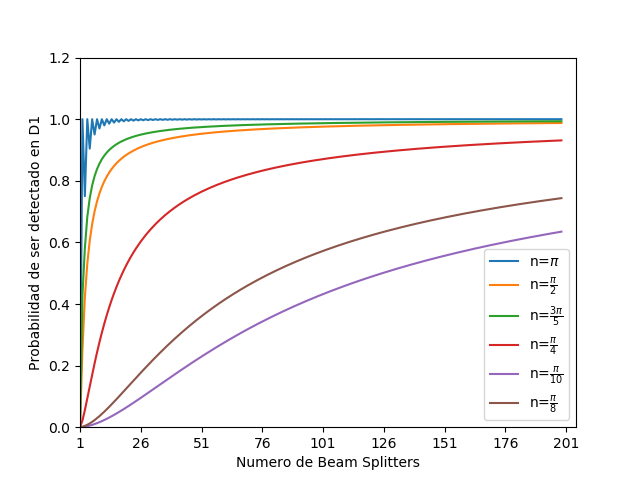
\includegraphics[width=\linewidth,height=5 cm]{images/BS_Azuna.png}
\caption{$P_{D_{1}}$}
\label{fig:BS1}
\end{subfigure}
\begin{subfigure}[b]{0.45\linewidth}
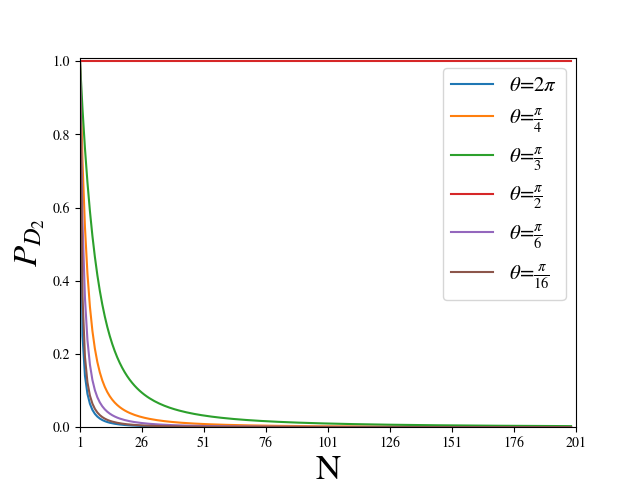
\includegraphics[width=\linewidth,height=5 cm]{images/BS_AzunaD2.png}
\caption{$P_{D_{2}}$}
\label{fig:westminster_aerea}
\end{subfigure}
\begin{subfigure}[b]{0.45\linewidth}
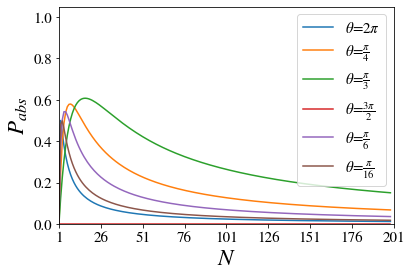
\includegraphics[width=\linewidth,height=5 cm]{images/absorbido_azuna.png}
\caption{$P_{abs}$}
\label{fig:BS1}
\end{subfigure}
\caption{Detection probabilities for an array with $\Theta=\frac{\pi}{2N}$, the detection probability in $D_{1}$ (a), $D_{2}$ (b) or that the photon will be ``lost'' (c). }
\label{Azuma1}
\end{figure}


Fig. \ref{Azuma1} shows different probabilities as we increase $N$. We can see that the probability of detection in $D_{1}$ asymptotically approaches one as Azuma had shown \cite{Azuma}. By substituting the bombs with beam splitters, we obtained similar results. Moreover, if we want to perform the experiment varying continuously the transitivity of the obstacle, we can use a polarizer and analyzer \cite{leonhartd}.  The case of a $BS$ is described by the same mathematics that an analyzer and a polarizer \cite{leonhardt}, unlike other absorbers this can be manipulated continually, giving us a way to test these curves experimentally.

 \section{Using identical beam splitters for all $N$}
 
In the previous section, each time we consider a different number $N$ of beam splitters, we needed to change $\Theta = \frac{\pi}{2N}$. But, one may wonder  how the system behaves for growing $N$ but fixed $\Theta$, maybe we could make the probability of detecting in $D_{1}$ grow as well, but after the analysis. We can see that even though it may grow for low $N$ it soon begins to lower and approaches zero very quickly the different values we tested. As Fig. \ref{Azuma2} shows.


\begin{figure}[!t]
\centering
\begin{subfigure}[b]{0.45\linewidth}
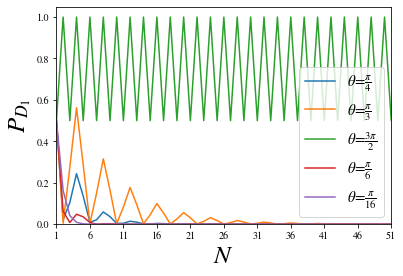
\includegraphics[width=\linewidth]{images/BsFijo_azumaD1.png}
\caption{$P_{D_{1}}$}
\label{fig:BS1}
\end{subfigure}
\begin{subfigure}[b]{0.45\linewidth}
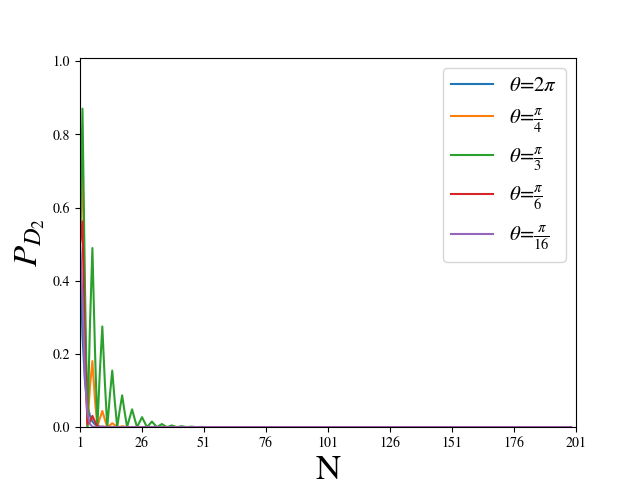
\includegraphics[width=\linewidth]{images/BsFijo_azumaD2.png}
\caption{$P_{D_{2}}$}
\label{fig:westminster_aerea}
\end{subfigure}
\begin{subfigure}[b]{0.45\linewidth}
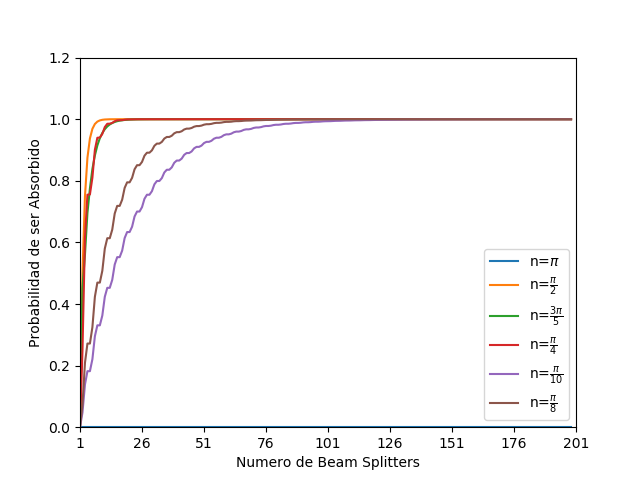
\includegraphics[width=\linewidth]{images/BsFijo_azumaabs.png}
\caption{$P_{abs}$}
\label{fig:BS1}
\end{subfigure}
\caption{Behavior for growing $N$ 50:50 $BS$ for all $N$,we show the probability of detection in $D_{1}$(a), $D_{2}$(b) and the probability of the photon being ``lost'' (c).}
\label{Azuma2}
\end{figure}





 
 Fig. \ref{Azuma2} shows the probabilities when we increase the number of $BS$ but do not change the transmitivity of them as $N$ increases. This may seem like a waste of effort since the aim is to maximize the detection probability. However, let us assume that we have an absorber that has a very little absorption probability, if we wanted to have it absorbing our photon this scheme would prove useful

\section{Using different beam splitters}

As we explored at the beginning of this chapter what gives us distinguishability between the case where we have an object in one of the arms of the interferometer and when there is no obstacle is the fact that when the sum of the angles is $\frac{ \pi}{2}$ so that when no object is there the output will be in detected in the opposite path when sent the photon in.

Could we use different angles that sum up to $\frac{\pi}{2}$? and still, enhance the probability of detection in $D_{1}$. The answer is yes, to illustrate it let us remember that the probability of detection in $D_{1}$ is given by Eq. \ref{comentatio}

\begin{equation*}
P_{D_{1}}=|\bra{2} (B \times A)^{N-1}B \ket{2}|^2
\end{equation*}

As we stated in section 2.2 the problem was reduced to matrix multiplication so we can get $P_{D_{1}}$ in this fashion, to illustrate the point, let us fix $N$, let us use $N=3$ then $P_{D_{1}}$ is given by:
\small
\begin{align*}
&P_{D_{1}}=\beta^{4} \sin^{2}{\left(\theta_{1} \right)} \sin^{2}{\left(\theta_{3} \right)} \cos^{2}{\left(\theta_{2} \right)} + 2 \beta^{3} \sin{\left(\theta_{1} \right)} \sin{\left(\theta_{2} \right)} \sin{\left(\theta_{3} \right)} \sin{\left(\theta_{1} + \theta_{3} \right)} \cos{\left(\theta \right)} \cos{\left(\theta_{2} \right)} \\
 & - 2 \beta^{2} \sin{\left(\theta_{1} \right)} \sin{\left(\theta_{3} \right)} \cos{\left(2 \theta \right)} \cos{\left(\theta_{1} \right)} \cos^{2}{\left(\theta_{2} \right)} \cos{\left(\theta_{3} \right)} + \beta^{2} \sin^{2}{\left(\theta_{2} \right)} \sin^{2}{\left(\theta_{1} + \theta_{3} \right)} \\
 & - 2 \beta \sin{\left(\theta_{2} \right)} \sin{\left(\theta_{1} + \theta_{3} \right)} \cos{\left(\theta \right)} \cos{\left(\theta_{1} \right)} \cos{\left(\theta_{2} \right)} \cos{\left(\theta_{3} \right)} + \cos^{2}{\left(\theta_{1} \right)} \cos^{2}{\left(\theta_{2} \right)} \cos^{2}{\left(\theta_{3} \right)}
\end{align*}
\normalsize

where $\beta$ is the transparency of the object and $\theta$ the phase it induces, now let us see what happens in the case we expect the most absorption ($\beta=0$) 

\begin{equation}
P_{D_{1}}=\cos^{2}{\left(\theta_{1} \right)} \cos^{2}{\left(\theta_{2} \right)} \cos^{2}{\left(\theta_{3} \right)}
\end{equation}

If we make $\theta_{i}=\frac{\pi}{2N}$ just like at the beginning of this chapter then

\begin{equation}
P_{D_{1}}=\cos^{6}{\left(\frac{\pi}{6} \right)}=\frac{27}{64}=0.421875
\end{equation} 

But if instead, we preserve that the sum is $\frac{\pi}{2}$,  but we use different angles we can achieve a lower probability of detection for lower $N$, let us show this by using $\theta_{1}=\frac{\pi}{4}$, $\theta_{2}=\frac{\pi}{6}$ and $\theta_{3}=\frac{\pi}{12}$ then 

\begin{equation}
P_{D_{1}}=\cos^{2}{\left(\frac{\pi}{4} \right)} \cos^{2}{\left(\frac{\pi}{6} \right)} \cos^{2}{\left(\frac{\pi}{12} \right)}=0.3499
\end{equation}

Now, What happens for higher $N$? this analysis remains the same, this happens because as Kwait et al \cite{exp} reasoned if the photon is to be detected then it always was reflected so it did not interact with the object and we simply have the product of cosines. If we get analytic answers and set $\beta=0$ then we get the same answer as they did with their reasoning, If we have semitransparent objects then we just as we can see from the curves in the previous section a semitransparent object reduces our probability of detecting in $D_{1}$ as we can also see plotting the analytical answer vs $\beta$.

\begin{figure}[!t]
\centering
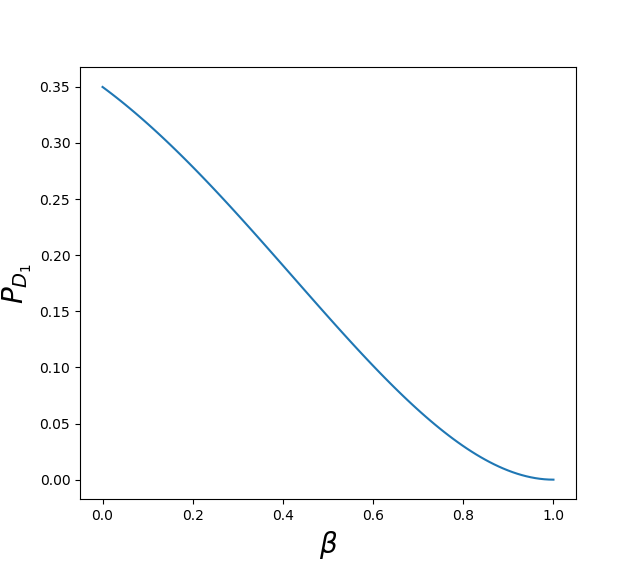
\includegraphics[scale=0.5]{images/alonso_idea.png}
\caption{Behaviour of the probability when we use different angles as we vary $\beta$ for $N=3$, we used $\theta_{1}=\frac{\pi}{4}$,$\theta_{2}=\frac{\pi}{6}$ and $\theta_{3}=\frac{\pi}{12}$ .}
\end{figure}

From this analysis, we can conclude that the best bomb detector we could build would be one whose bomb is perfectly absorbent and whose beam splitters use $\Theta=\frac{\pi}{2 N}$. However, in practice, such an object is difficult to obtain and that is why models with semitransparent objects are useful.
 
\section[Optical chopper]{Optical chopper as imperfect absorber in $N$ interferometers}

In this next section, we will replace the $N-1$ imperfect absorbers by $N-1$ sinchronized identical optical choppers.For an optical chopper the following matrix could be used:

\begin{equation}
A_{chopper}=\begin{pmatrix} f & 0 \\ 0 & 1 \end{pmatrix}.
\end{equation}

However, as $f$ only varies discretely our matrix will alternate between  two transparencies ($\beta$ and 1):

\begin{equation}
f=\left(\frac{1-sgn(\sin(wt))}{2} \right)\beta+\frac{1+sgn(\sin(wt))}{2}.
\end{equation}

In the positive cycle we have $f=1$. While on the negative cycle $f=\beta$. For convenience, we will rewrite the matrix in Eq. \ref{absorber} in terms of $|\beta|$, this way in the positive cycle we will have the case of the nested interferometer with no object which is the same as  $\beta=1$, but in the negative cycle, we will have  Azuma's case.


 \begin{figure}[!t]
\centering
\begin{subfigure}[b]{0.45\linewidth}
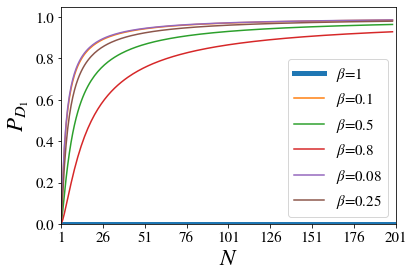
\includegraphics[width=\linewidth]{images/ChopperD1.png}
\caption{$P_{D_{1}}$}
\label{fig:BS1}
\end{subfigure}
\begin{subfigure}[b]{0.45\linewidth}
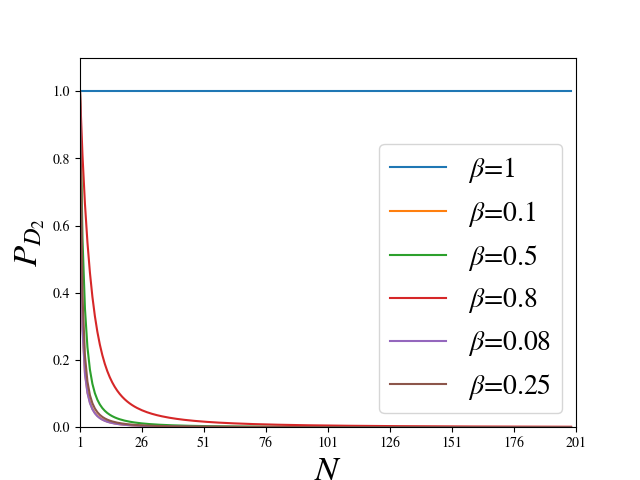
\includegraphics[width=\linewidth]{images/ChopperD2.png}
\caption{$P_{D_{2}}$}
\label{fig:westminster_aerea}
\end{subfigure}
\begin{subfigure}[b]{0.45\linewidth}
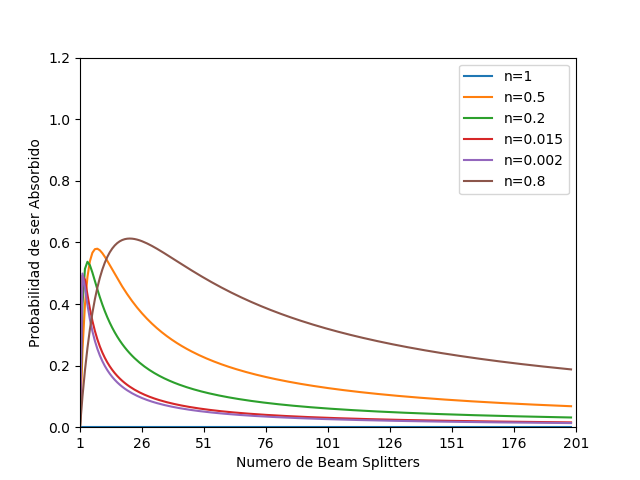
\includegraphics[width=\linewidth]{images/Chopper_abs.png}
\caption{$P_{abs}$}
\label{fig:BS1}
\end{subfigure}
\caption{Behavior for growing $N$ for optical choppers as imperfect absorbers, (a) shows the probability of detection in $D_{1}$, (b) the probability of detection in $D_{2}$ and (c) the probability of the photon being ``lost''.}
\label{fig:several_chpper}
\end{figure}
 

Fig. \ref{fig:several_chpper} shows the probabilities distributions for optical choppers with different transparencies, the blue line represents the ``hole" part of the chopper, and the other lines represent the ``material" part, the system will alternate periodically between these probabilities.

\section{Does the phase matter?}

As we saw in the previous section, if we use nested interferometers we can increase the probability of detecting in $D_{1}$ arbitrarily close to unity, (if we put the semitransparent objects in the other arm the opposite is true). However, neither in the treatment by Azuma \cite{Azuma} nor in the previous section the phase the object induces was considered, only its transmission coefficient. Is it unimportant?

To answer that question we explore how the object inducing a phase would affect our previous calculations. To introduce it, one simply modifies Eqs. \ref{absorber} or \ref{absorber1}. by multiplying $\beta$ by a phase (equivalent to considering a phase shifter in the same arm the object is in). the resulting matrix is:

\begin{equation}
 A=\begin{pmatrix} \beta e^{i \theta}& 0\\0&  1\end{pmatrix}.
 \end{equation}

By doing the same procedure as in section 6.1, we plot $P_{D_{1}},P_{D_{2}},P_{abs}$ vs. $\theta$ fixing $N$. 

\begin{figure}[!t]
\centering
\begin{subfigure}[b]{0.30\linewidth}
\includegraphics[width=\linewidth]{images/Azuma_phases2.png}
\caption{$N=2$}
\end{subfigure}
\begin{subfigure}[b]{0.30\linewidth}
\includegraphics[width=\linewidth]{images/Azuma_phases5.png}
\caption{$N=5$ }
\label{fig:BS1}
\end{subfigure}
\begin{subfigure}[b]{0.30\linewidth}
\includegraphics[width=\linewidth]{images/Azuma_phases10.png}
\caption{$N=10$ }
\label{fig:BS1}
\end{subfigure}
\begin{subfigure}[b]{0.30\linewidth}
\includegraphics[width=\linewidth]{images/Azuma_phases100.png}
\caption{$N=100$}
\end{subfigure}
\begin{subfigure}[b]{0.30\linewidth}
\includegraphics[width=\linewidth]{images/Azuma_phases1000.png}
\caption{$N=1000$ }
\label{1000}
\end{subfigure}
\caption{Behaviour of probabilities as $N$ grows and we vary $\theta$ for $\beta=0.5$, (a) $N$=2,(b) $N$=5,(c) $N$=10,(d) $N$=100,(e) $N$=1000.}
\label{con_fase}
\end{figure}

As we see from Fig. \ref{con_fase} the phase is important when $N$ is small but as $N$  grows the dependence on the phase $\theta$ becomes smaller until we see for example in Fig \ref{1000} when $N$ is big. It is almost constant with the variation of $\theta$.

These plots, allow us to know the phases that would improve our bomb detector for unbalanced interferometers (an unbalanced interferometer is one with misalignments), such as the one developed in \cite{Chao_2018} for any given transparency and number of beam spliters.


\section{Towards Wheeler's Gedanken experiment}

One of the main reasons the Mach-Zehnder interferometer is so popular is that it allows us to study fundamental facts about quantum theory such as Bohr's complementary principle, this is well explained in \cite{delayed}. It consists in wondering if a photon behaves like a particle or a wave in a Mach-Zehnder interferometer, the idea is better explained with the following the Gedanken experiment.

\begin{figure}[H]
\centering
\includegraphics[width=\linewidth,height=6.5 cm]{images/wheeler1.png}
\caption{Mach-Zehnder interferometer with both $BS$ being 50:50, we always detect on $D_{1}$.}
\label{wheeler1}
\end{figure}

Let us picture a Mach-Zehnder interferometer like the one shown in Fig. \ref{wheeler1}, let both $BS$ be 50:50, now let us also imagine that we send in a single photon, from the section 3.2 we get Eq. \ref{pp_wheler}, if the difference in the optical path is $\gamma_{1}-\gamma_{2}=0$  we get certainty of where the detection will be made ($D_{1}$), however, we have no information of which path the photon took.

\begin{figure}[H]
\centering
\includegraphics[width=\linewidth,height=6.5 cm]{images/wheeler2.png}
\caption{Mach-Zehnder interferometer without the second $BS$.}
\label{wheeler2}
\end{figure}

Now, let us consider the new arrangement shown in Fig. 6.8, as it is shown in Fig. \ref{wheeler2} where we removed the second beam splitter from the interferometer. This time we have no certainty of where the photon detection is going to be made (it is split with equal probability to $D_{1}$ and $D_{2}$), however, once we detect the photon we have complete information of which path the photon took.



In one setting, we have wave-like behavior and in the other, we have partcile-like behavior. In the wheeler Gedanken experiment, the idea is to have the second beam splitter in a superposition of being there or not. It seems that before entering the experiment the photon somehow decides whether it is going to behave as a particle or as a wave, which seems to be in accordance with Bohr's complementary principle. This is precisely what quantum delayed-choice experiments seek to rule out \cite{Ma}, where the photon has particle or wave behavior or even a continuous transition between these two very different behaviors while the experiment is running.

\begin{figure}[H]
\centering
\includegraphics[width=\linewidth,height=7.5 cm]{images/wheeler3.png}
\caption{Mach-Zehnder interferometer with the second $BS$ is a in a superposition of being and not being.}
\label{wheeler3}
\end{figure}

It was recently demonstrated \cite{Peruzzo, Kaiser2012} that there is a smooth transition between particle and wave behaviors thus Bohr's complementary principle seems to be invalid. The way they did this experiment was through a very clever implementation of the original Gedanken experiment where we have a ``Quantum'' $BS$, which is a $BS$ that is in a superposition state of being there and not being there as in Fig. \ref{wheeler3}. They achieved this superposition was by implementing a controlled Hadarmard gate \footnote{As was discussed in the beam splitter section a Hadamard gate is equivalent to a 50:50 beam splitter}, acting as an identity gate if a control qubit is in the $0$ state and as a Hadamard gate if the control qubit is in the $1$ state.  If the control qubit is in a superposition state, so will be the controlled Hadamard gate.




A similar situation arises through interaction-free measurements, since taking a path means interacting with the object, and taking the other path means no interaction, thus we have some sort of controlled gate. The first $BS$ puts the photon in a superposition of both paths (note that this approach differs significantly from the one taken in \cite{Peruzzo,Kaiser2012} because our $BS$ differ from a Hadamard gate by more than a phase, this approach is more controllable ), and then both paths are recombined in the second $BS$, recall we always have the second beam splitter on as the experiments proposed recently do \cite{Polino}.

\begin{figure}[H]
\centering
\begin{subfigure}[b]{0.40\linewidth}
\includegraphics[width=\linewidth]{images/pd1_2.png}
\caption{$P_{D_{1}}$}
\end{subfigure}
\begin{subfigure}[b]{0.40\linewidth}
\includegraphics[width=\linewidth]{images/pd2_2.png}
\caption{$P_{D_{2}}$ }
\label{fig:BS1}
\end{subfigure}
\begin{subfigure}[b]{0.40\linewidth}
\includegraphics[width=\linewidth]{images/pabs_2.png}
\caption{$P_{D_{2}}$ }
\label{fig:BS1}
\end{subfigure}
\caption{Continuos transition between wave and particle behaviour with 50:50 $BSs$, (a) shows the probability that the photon is detected at $D_{1}$,(b) at $D_{2}$ and (c) the probability the photon is ``lost''.}
\label{transzuri}
\end{figure}

If, we have both $BS$ in the setup, how can the transition between particle and wave behavior be achieved? The answer is simple, the object introduces two new parameters that can be tuned to change the behavior of the photon from particle to wave since these properties change the probabilities at the output as was studied in previous sections. This was studied by Zurika Blanco-Garcia and Oscar Rosas-Ortiz in \cite{azuri} for the 50:50 $BS$ case. Those plots are in perfect agreement with the experiments. However, no experimental realization has been done in this setup. Fig. \ref{transzuri} shows the transition from particle to wave behavior in the 50:50 case. (To make it more comparable to experiments we included the effect of misalignment $\gamma_{1},\gamma_{2}$, in the output they end up in a sum with the phase of the object, we included this in a single parameter $\Delta$):

\begin{figure}[H]
\centering
\begin{subfigure}[b]{0.40\linewidth}
\includegraphics[width=\linewidth]{images/pd1_2_pi3.png}
\caption{$P_{D_{1}}$}
\end{subfigure}
\begin{subfigure}[b]{0.40\linewidth}
\includegraphics[width=\linewidth]{images/pd2_2_pi3.png}
\caption{$P_{D_{2}}$ }
\label{fig:BS1}
\end{subfigure}
\caption{Continuous transition between wave and particle behavior with 25:75 BSs the probability of detection in $D_{1}$ is shown in (a) and for $D_{2}$ in (b)}
\label{pi/3}
\end{figure}


 we do not need to restrict ourselves to the 50:50 case, other cases even though present the same shape as Fig. \ref{pi/3} they do it from different values of the parameters allowing us to test this beyond the 50:50 beam splitters.

\begin{figure}[H]
\centering
\begin{subfigure}[b]{0.45\linewidth}
\includegraphics[width=\linewidth]{images/pd1_3_pi4.png}
\caption{$P_{D_{1}}$}
\end{subfigure}
\begin{subfigure}[b]{0.45\linewidth}
\includegraphics[width=\linewidth]{images/pd2_3_pi4.png}
\caption{$P_{D_{2}}$ }
\label{fig:BS1}
\end{subfigure}
\begin{subfigure}[b]{0.45\linewidth}
\includegraphics[width=\linewidth]{images/pabs_3_pi4.png}
\caption{$P_{D_{2}}$ }
\label{fig:BS1}
\end{subfigure}
\begin{subfigure}[b]{0.45\linewidth}
\includegraphics[width=\linewidth]{images/pd1_5_pi4.png}
\caption{$P_{D_{1}}$ }
\label{fig:BS1}
\end{subfigure}
\begin{subfigure}[b]{0.45\linewidth}
\includegraphics[width=\linewidth]{images/pd2_5_pi4.png}
\caption{$P_{D_{2}}$ }
\label{fig:BS1}
\end{subfigure}
\begin{subfigure}[b]{0.45\linewidth}
\includegraphics[width=\linewidth]{images/pabs_5_pi4.png}
\caption{$P_{D_{2}}$ }
\label{fig:BS1}
\end{subfigure}
\caption{Continuous transition between wave and particle behaviour with 50:50 $BSs$ for $N=3$ and $N=5$. The top plots correspond to $N=3$ they show the probability of detection in $D_{1}$ (a),$D_{2}$ (b) and the probability of the photon being ``lost''(c). The botton plots correspond to $N=$ they show the probability of detection in $D_{1}$ (d),$D_{2}$ (e) and the probability of the photon being ``lost'' (f)}
\label{varias}
\end{figure}

Now, let us consider a high efficiency Mach-Zehnder interferometer with $N$ beam splitters. We get multiple transitions as Fig. \ref{varias} shows, there we can see the plots for $N=3$ and $N=5$, in theses plots we consider all objects in the interferometer to be equal, we also considered all beam splitters to be 50:50 and we dropped the general form of the mirrors, selecting $\gamma_{1}=\gamma_{2}=\frac{\pi}{2}$), as we can see we have more than one transition between particle and wave behavior, however, we see that this happens only for $\beta \approx 1$ which may suggest that the transition only happens for almost transparent or transparent objects. However, this is because the absorption probability tends to $1$ as $N$ grows as we showed in section 6.1

We can circumvent this by using $BS$ with $\Theta=\frac{\pi}{2N}$, exploiting the quantum Zeno effect as explained in the previous section, we could then see more interesting transitions, and we get plots like the ones in Fig. \ref{figvarias2}, all other parameters are maintained.

A more general complementary principle is formulated with regard to this experiments \cite{Ma}, this one is an inequality and goes as:

\begin{equation}
 V^{2} + D^{2} \leq 1,
\end{equation}

where $V$ is the visibility, $D$ is the distinguishability and are defined as :

\begin{align}
 V= \frac{P_{max}-P_{min}}{P_{max}+P_{min}}\\
 D_{i}=|p(i,1)-p(i,2)|
\end{align}


\begin{figure}[H]
\centering
\begin{subfigure}[b]{0.45\linewidth}
\includegraphics[width=\linewidth]{images/pd1_3.png}
\caption{$P_{D_{1}}$}
\end{subfigure}
\begin{subfigure}[b]{0.45\linewidth}
\includegraphics[width=\linewidth]{images/pd2_3.png}
\caption{$P_{D_{2}}$ }
\label{fig:BS1}
\end{subfigure}
\begin{subfigure}[b]{0.45\linewidth}
\includegraphics[width=\linewidth]{images/pabs_3.png}
\caption{$P_{D_{2}}$ }
\label{fig:BS1}
\end{subfigure}
\begin{subfigure}[b]{0.45\linewidth}
\includegraphics[width=\linewidth]{images/pd1_5.png}
\caption{$P_{D_{1}}$ }
\label{fig:BS1}
\end{subfigure}
\begin{subfigure}[b]{0.45\linewidth}
\includegraphics[width=\linewidth]{images/pd2_5.png}
\caption{$P_{D_{2}}$ }
\label{fig:BS1}
\end{subfigure}
\begin{subfigure}[b]{0.45\linewidth}
\includegraphics[width=\linewidth]{images/pabs_5.png}
\caption{$P_{D_{2}}$ }
\label{fig:BS1}
\end{subfigure}
\caption{Continuous transition between wave and particle behaviour with $\theta=\frac{\pi}{2N}$ $BS$s for $N=3$ and $N=5$. The top plots correspond to $N=3$ they show the probability of detection in $D_{1}$ (a),$D_{2}$ (b) and the probability of the photon being ``lost''(c). The bottom plots correspond to $N=5$, they show the probability of detection in $D_{1}$ (d),$D_{2}$ (e) and the probability of the photon being ``lost'' (f)}
\label{figvarias2}
\end{figure}




where $P_{max}$ and $P_{min}$ refer to the maximal and minimal for recording a photon in a chosen detector when scanning through the phase of the interferometer. The distinguishability or which-path information is defined as $D=D_{1}+D_{2}$ and $p(i,j)$ the probability that the photon travelled the path $i=1,2$ and arrived at detector $j=1,2$.


In conclusion, we proposed a simpler way to get the transition from wave and particle behavior, as \cite{Kaiser2012,Peruzzo} uses sophisticated equipment to implement a controlled Hadamard gate, we proposed a simpler scheme to achieve the same results both theoretically and experimentally. Besides requiring this complicated implementations a lot of debate has been arising since some claim that the experiments in \cite{Peruzzo,Kaiser2012}  can be explained with a two-dimensional classical variable \cite{Rossi,Chaves}, recently a proposal and implementation for an experiment that could not be explained in this way was presented in \cite{Polino}.





\pagebreak







\pagebreak
\chapter{Experimental Setup}
In this chapter, we will describe the necessary materials and steps to realize all of the previous content of this thesis experimentally. All of the work from this section on took place at the laboratory for quantum and electromagnetic phenomena at UPIITA. We will begin by generating a single photon source using SPDC, we will follow the approach taken in \cite{maestria_procopio}. We will then replicate the Elitzur-Vaidman ``bomb detector''. Finally, we will study variations of this ``bomb detector'' with semitransparent objects.

\section{Single-photon source}


To produce a single-photon source we will use the SPDC process described in chapter 1, to do this experimentally we will follow the method described in \cite{maestria_procopio}. The experimental setup can be seen .in Fig. \ref{single}.  We will use the following materials:



\begin{itemize}

\item Aluminum rails
\item Infrared filters 810nm $\pm$ 10nm
\item Violet laser 405nm
\item Pinholes
\item BBO-I crystal
\item Multimode optical fiber
\item APDs(Avalanche photo-diodes)
\item National instruments' data acquisition board
\item Newport posts
\item Optical Table

\end{itemize}

\begin{figure}[H]
\centering
\includegraphics[width=\linewidth]{images/SPDC_exp.png}
\caption{Experimental setup of single photon source}
\label{single}
\end{figure}

The first step to achieve a single photon source is to find the most likely light-cone using individual counts in each photo-detector as described in chapter 2 section 2.1 where we explained type-I SPDC, after that, we need to count coincidences to identify spatial correlations as described in chapter 1. We will set the detection window for coincidences based on the procedure of \cite{pearson} at 10ns, this coincidence window is used so we know the pair of photons are created in the nonlinear crystal thus eliminating noise from the environment in the detection counts. It is usually convenient for the propagation direction of the photon to be co-lineal with one of the lines of tapped holes

In BBO-I crystals both photons have the same energy, from Eq. \ref{conservation} we can see that this implies that both signal and idler photons' direction of propagation makes the same angle with respect to the direction of the laser beam as seen in Fig. \ref{single}.

Since we know the relationship between each of the propagation directions, and it is in our best interest to have the signal photon co-lineal to the tapped holes, we will make the necessary adjustments so this happens. This is usually done by first setting the laser pump to be co-linear to the tapped holes, and then rotating both the laser and the crystal in such a way that the laser propagates in the direction previously occupied by the idler photon while the signal photon propagates in the direction previously occupied by the laser. The new direction of the idler photon can be found using Eq. \ref{conservation}.

Once we achieve this, we place APDs in the direction of propagation of both signal and idler photons. Our single-photon source is ready to go and the next step we need to take is to set up and align the Mach-Zehnder interferometer.

\section{Single-photon Mach-Zehnder interferometer}

As we previously described in chapter 1, the Mach-Zehnder interferometer is made of two beam splitters ($BS_{1}$ and $BS_{2}$) and two mirrors($M_{1}$ and $M_{2}$). As the Eliztur-Vaidman ``bomb detector'' uses $50:50$ beam splitters and that's a result we want to replicate we will set up our interferometer using those. In addition to the previous section we will need:

\begin{itemize}
\item Two 50:50 Beam splitters
\item Two mirrors
\item Red laser 700nm
\item Incandescent white light source
\item Piezoelectric Thorlabs AE0505D-16F
\end{itemize}

We aim to get the difference in optical paths to a minimum, that is we wish to achieve $|\gamma_{2}-\gamma_{1}|=0+2\pi n$, this alignment can be quite challenging in the laboratory. To achieve this we will consider the following approach for alignment as discussed in \cite{zuri}. To align the interferometer and reduce $|\gamma_{2}-\gamma_{1}|$ as much as possible, the strategy is to attach a piezoelectric device to one of the mirrors, align it by hand and then varying the voltage applied to the piezoelectric (changing this mirror's orientation) until a minimum is reached.

Both $D_{1}$ and $D_{2}$ are APDs placed in the same way as in Fig.1, in the output of  $BS_{2}$, the interference pattern requires special treatment of the counts since unlike the classical case where we inject coherent beams into the interferometer we are injecting single photons. This ``special treatment'' consists in only considering detector clicks when there's a simultaneous coincidence in $D_{idler}$, where $D_{idler}$ is an APD placed in the path of the idler photon as described in the SPDC section, we will use the same temporal window of ``simultaneously'' as described in the previous section that is 10ns. The experimental set up for this section is shown in Fig. \ref{newsingle}.


\begin{figure}[H]
\centering
\includegraphics[width=\linewidth]{images/machzehnder_single.png}
\caption{Experimental setup of a single photon Mach-Zehnder Interferometer}
\label{newsingle}
\end{figure}

\subsection{Alignment of the Interferometer}

In this section, we will describe in detail the procedure used to align the Mach-Zehnder interferometer this approach was used in \cite{zuri}, as mentioned before the idea is to get $|\gamma_{2}-\gamma_{1}|=2\pi n$. It is necessary to be meticulous regarding the optical devices' position and characteristics, for instance, it is necessary to consider that the $BS$ faces are not completely flat, this is a problem because a $BS$ can change the propagation direction of the transmitted beam even when placed at $\theta=45\degree$. We will use $BS_{1}=BS_{2}=50:50$

To align the interferometer we begin by placing a red laser(HeNe) in such a way that the beam goes through the same path as the signal photon did in Fig. \ref{single}. To do this two collimators are needed. One is placed as close as possible to the BBO-I crystal, and the other one is placed near the $D_{signal}$ from the SPDC array. All alignment of our Mach-Zehnder interferometer is done using this red laser. In Fig.19 (a-d) all the steps we are going to take to align the interferometer are shown.

\begin{figure}[H]
\centering
\begin{subfigure}[b]{0.55\linewidth}
\includegraphics[width=8cm,height=4 cm]{images/first_step.png}
\caption{First step}
\label{fig:BS1}
\end{subfigure}
\begin{subfigure}[b]{0.55\linewidth}
\includegraphics[width=8cm,height=4 cm]{images/second_step.png}
\caption{Second step}
\label{fig:BS1}
\end{subfigure}
\begin{subfigure}[b]{0.55\linewidth}
\includegraphics[width=8cm,height=4 cm]{images/third_step.png}
\caption{Third step}
\label{fig:BS1}
\end{subfigure}
\begin{subfigure}[b]{0.55\linewidth}
\includegraphics[width=8cm,height=4 cm]{images/last_step.png}
\caption{Fourth and last step}
\label{fig:westminster_aerea}
\end{subfigure}
\caption{Steps to align the Mach-Zehnder interferometer}
\label{steps}
\end{figure}



The first step is to place $BS_{1}$ at $\theta=45\degree$ with respect to the incoming beam so it is placed in its optimal position and does not deviate the beam. Additionally, both the transmitted and reflected beam must be co-linear to the tapped holes in the optical table. Using two screens we will mark where both the transmitted and reflected photons go as shown in Fig. \ref{steps} (a-d).

The second step is to place one of the mirrors $M_{2}$ in the path of the transmitted beam, the idea is to place $M_{2}$ in such a way that the reflected beam is co-lineal with the tapped holes of the optical table, and then mark on the screen the place where the beam goes, as is shown in Fig. \ref{steps}(b).

The third step is to dismount $M_{2}$(Only the mirror it isn't necessary to take out the post) and to place $M_{1}$ and repeat the step to using $M_{1}$ instead of $M_{2}$. We will place one of the mirrors in a ¿post? with a micro-metric screw and piezoelectric device to obtain vertical mobility, We will choose $M_{1}$, after completing this step we place $M_{2}$ once again, the expected result so far is shown in Fig. \ref{steps}(c).

The fourth and last step is to place $BS_{2}$ as it is shown in Fig. \ref{steps}(d), the reflected and transmitted beam should reach the marks done in step three, since we are working with a coherent beam we will see the interference pattern achieved on the screen. Once we have achieved the desired interference pattern, this same setup should be tested with white light from an incandescent source, that is because the coherence-length of the red laser is very long, so it is relatively easy to get red interference, therefore, using red light and getting an interference pattern is not such a precise test of alignment. When using white light it is way harder to get interference patterns visible, it requires a much finer alignment. After we have tested with white light, we will place the APDs on the marks that correspond to the mirrors' reflected beams.


We should make the Mach-Zehnder interferometer as small as possible, this allows better control over the length of the optical paths making alignment easier.

\subsection{Single-photon interference}

Once we've done all of this we are ready to start the experiments that mainly concern this thesis, we will begin by replicating the ``Elitzur-Vaidman'' experiment, and then move on to the variations with semitransparent objects.


\begin{itemize}
\item {\large \textbf{Perfect absorber}}
\end{itemize}
To have an imperfect absorber we will use a polarizer and an analyzer since we are using type-I SPDC (we are using a BBO-I crystal) we know that both the signal and idler photon will have identical polarizations and that it will be orthogonal to that of the photon. We can fabricate a perfect absorber by rotating the analyzer. This is because as Malus' law states \cite{hecht}

\begin{equation}
I=I_{0} \cos^{2}(\theta)
\end{equation}

where $I_{0}$ is the intensity before the polarizer and analyzer, $I$ is the intensity after them, and $\theta$ is the angle between the polarizer and analyzer if we rotate them in such a way that $\theta=0$ then we have our perfect absorber that can be placed in one of the arms of our interferometer


The Quantum version of this law is very similar \cite{malus} a generalization for fermions was also obtained. Therefore this analogy is valid both in the classical and quantum regime.
 \begin{itemize}
\item {\large \textbf{Semitransparent Objects}}
\end{itemize}

The behavior of a $BS$ is analogous to that of an analyzer and polarizer(same transmission and reflection/absorption coefficients) as Leonhartd states in \cite{Leonhardt_2003} a pictorial diagram of the analogy is shown in Fig. \ref{BS and polarizer}, so to get a fair number of experimental points in the $BS$ as imperfect transmitter curves, we will use a polarizer and analyzer and vary $\theta$, the ``lost'' photon will be absorbed instead. The same idea will be used for the $N$ beam-splitter section. Curves will be made once we know with how many we can count in the laboratory, that way setting $N$.

\begin{figure}[H]
\centering
\includegraphics[width=\linewidth]{images/polarizeranalogy.png}
\caption{Polarizer and analyzer analogy}
\label{BS and polarizer}
\end{figure}

An interesting experiment that could be replicated and generalized if time allows is the realization of ``$N$ interferometers'' as Kwait et al. realized in \cite{exp}, whereby taking advantage of this analogy and exploiting the quantum Zeno effect \cite{zeno} designed a version of this experiment that requires just a few optical devices, a semitransparent object could be placed in this setup enabling us to compare with the curves in section 5.


In the case of the chopper, one with perfect absorption would be quite difficult to implement, therefore this curves may not be tested and remain pending work, in the case of the chopper as an imperfect absorber the idea is to 3D print an optical chopper that is hollow and can be filled with different powders and liquids, changing its optical properties, the downside of this approach is that every time we fill it with something different its optical properties must be characterized.



\subsection{Varying optical paths}

To be able to see the interference pattern, it is necessary to adjust the difference in optical paths $\delta \phi$. Visibility is a quantitative measure of the quality of the interference pattern, classically it is defined as \cite{hecht}:

\begin{equation}
V=\frac{I_{max}-I_{min}}{I_{max}+I_{min}},
\end{equation}

where $I_{max}$ is the maximum intensity and $I_{min}$ is the minimum intensity of the interference pattern. The ideal pattern has perfect visibility ($V$=1), which happens when $I_{min}=0$.

In quantum mechanics the intensity is proportional to the expected value of the photon number \cite {glauber}, so the visibility is then given by:

\begin{equation}
V=\frac{N_{max}-N_{min}}{N_{max}+N_{min}},
\end{equation}

In the lab $N_{max}$ and $N_{min}$ correspond to the maximum and minimum coincidences $D_{1}-D_{idler}$ as we vary the voltage on the piezoelectric device.

Visibility counts will vary as we change the difference in optical paths $\delta\phi$ by varying the voltage on the piezoelectric attached to the mirror, the idea is to see how visibility changes with voltage and keep the maximum value that we can achieve to keep going with the rest of the experiments.
  
\pagebreak






 
\chapter*{Conclusions}
\thispagestyle{plain}

\pagebreak
\addcontentsline{toc}{chapter}{Conclusions}


\bibliographystyle{unsrt}
\bibliography{bibliography}


\end{document}





